% Options for packages loaded elsewhere
\PassOptionsToPackage{unicode}{hyperref}
\PassOptionsToPackage{hyphens}{url}
%
\documentclass[
]{article}
\usepackage{lmodern}
\usepackage{amssymb,amsmath}
\usepackage{ifxetex,ifluatex}
\ifnum 0\ifxetex 1\fi\ifluatex 1\fi=0 % if pdftex
  \usepackage[T1]{fontenc}
  \usepackage[utf8]{inputenc}
  \usepackage{textcomp} % provide euro and other symbols
\else % if luatex or xetex
  \usepackage{unicode-math}
  \defaultfontfeatures{Scale=MatchLowercase}
  \defaultfontfeatures[\rmfamily]{Ligatures=TeX,Scale=1}
\fi
% Use upquote if available, for straight quotes in verbatim environments
\IfFileExists{upquote.sty}{\usepackage{upquote}}{}
\IfFileExists{microtype.sty}{% use microtype if available
  \usepackage[]{microtype}
  \UseMicrotypeSet[protrusion]{basicmath} % disable protrusion for tt fonts
}{}
\makeatletter
\@ifundefined{KOMAClassName}{% if non-KOMA class
  \IfFileExists{parskip.sty}{%
    \usepackage{parskip}
  }{% else
    \setlength{\parindent}{0pt}
    \setlength{\parskip}{6pt plus 2pt minus 1pt}}
}{% if KOMA class
  \KOMAoptions{parskip=half}}
\makeatother
\usepackage{xcolor}
\IfFileExists{xurl.sty}{\usepackage{xurl}}{} % add URL line breaks if available
\IfFileExists{bookmark.sty}{\usepackage{bookmark}}{\usepackage{hyperref}}
\hypersetup{
  pdfauthor={Alexandros Kokkalis, Elvar Halldor Hallfredsson, Lise Heggebakken},
  hidelinks,
  pdfcreator={LaTeX via pandoc}}
\urlstyle{same} % disable monospaced font for URLs
\usepackage[margin=1in]{geometry}
\usepackage{color}
\usepackage{fancyvrb}
\newcommand{\VerbBar}{|}
\newcommand{\VERB}{\Verb[commandchars=\\\{\}]}
\DefineVerbatimEnvironment{Highlighting}{Verbatim}{commandchars=\\\{\}}
% Add ',fontsize=\small' for more characters per line
\usepackage{framed}
\definecolor{shadecolor}{RGB}{248,248,248}
\newenvironment{Shaded}{\begin{snugshade}}{\end{snugshade}}
\newcommand{\AlertTok}[1]{\textcolor[rgb]{0.94,0.16,0.16}{#1}}
\newcommand{\AnnotationTok}[1]{\textcolor[rgb]{0.56,0.35,0.01}{\textbf{\textit{#1}}}}
\newcommand{\AttributeTok}[1]{\textcolor[rgb]{0.77,0.63,0.00}{#1}}
\newcommand{\BaseNTok}[1]{\textcolor[rgb]{0.00,0.00,0.81}{#1}}
\newcommand{\BuiltInTok}[1]{#1}
\newcommand{\CharTok}[1]{\textcolor[rgb]{0.31,0.60,0.02}{#1}}
\newcommand{\CommentTok}[1]{\textcolor[rgb]{0.56,0.35,0.01}{\textit{#1}}}
\newcommand{\CommentVarTok}[1]{\textcolor[rgb]{0.56,0.35,0.01}{\textbf{\textit{#1}}}}
\newcommand{\ConstantTok}[1]{\textcolor[rgb]{0.00,0.00,0.00}{#1}}
\newcommand{\ControlFlowTok}[1]{\textcolor[rgb]{0.13,0.29,0.53}{\textbf{#1}}}
\newcommand{\DataTypeTok}[1]{\textcolor[rgb]{0.13,0.29,0.53}{#1}}
\newcommand{\DecValTok}[1]{\textcolor[rgb]{0.00,0.00,0.81}{#1}}
\newcommand{\DocumentationTok}[1]{\textcolor[rgb]{0.56,0.35,0.01}{\textbf{\textit{#1}}}}
\newcommand{\ErrorTok}[1]{\textcolor[rgb]{0.64,0.00,0.00}{\textbf{#1}}}
\newcommand{\ExtensionTok}[1]{#1}
\newcommand{\FloatTok}[1]{\textcolor[rgb]{0.00,0.00,0.81}{#1}}
\newcommand{\FunctionTok}[1]{\textcolor[rgb]{0.00,0.00,0.00}{#1}}
\newcommand{\ImportTok}[1]{#1}
\newcommand{\InformationTok}[1]{\textcolor[rgb]{0.56,0.35,0.01}{\textbf{\textit{#1}}}}
\newcommand{\KeywordTok}[1]{\textcolor[rgb]{0.13,0.29,0.53}{\textbf{#1}}}
\newcommand{\NormalTok}[1]{#1}
\newcommand{\OperatorTok}[1]{\textcolor[rgb]{0.81,0.36,0.00}{\textbf{#1}}}
\newcommand{\OtherTok}[1]{\textcolor[rgb]{0.56,0.35,0.01}{#1}}
\newcommand{\PreprocessorTok}[1]{\textcolor[rgb]{0.56,0.35,0.01}{\textit{#1}}}
\newcommand{\RegionMarkerTok}[1]{#1}
\newcommand{\SpecialCharTok}[1]{\textcolor[rgb]{0.00,0.00,0.00}{#1}}
\newcommand{\SpecialStringTok}[1]{\textcolor[rgb]{0.31,0.60,0.02}{#1}}
\newcommand{\StringTok}[1]{\textcolor[rgb]{0.31,0.60,0.02}{#1}}
\newcommand{\VariableTok}[1]{\textcolor[rgb]{0.00,0.00,0.00}{#1}}
\newcommand{\VerbatimStringTok}[1]{\textcolor[rgb]{0.31,0.60,0.02}{#1}}
\newcommand{\WarningTok}[1]{\textcolor[rgb]{0.56,0.35,0.01}{\textbf{\textit{#1}}}}
\usepackage{longtable,booktabs}
% Correct order of tables after \paragraph or \subparagraph
\usepackage{etoolbox}
\makeatletter
\patchcmd\longtable{\par}{\if@noskipsec\mbox{}\fi\par}{}{}
\makeatother
% Allow footnotes in longtable head/foot
\IfFileExists{footnotehyper.sty}{\usepackage{footnotehyper}}{\usepackage{footnote}}
\makesavenoteenv{longtable}
\usepackage{graphicx,grffile}
\makeatletter
\def\maxwidth{\ifdim\Gin@nat@width>\linewidth\linewidth\else\Gin@nat@width\fi}
\def\maxheight{\ifdim\Gin@nat@height>\textheight\textheight\else\Gin@nat@height\fi}
\makeatother
% Scale images if necessary, so that they will not overflow the page
% margins by default, and it is still possible to overwrite the defaults
% using explicit options in \includegraphics[width, height, ...]{}
\setkeys{Gin}{width=\maxwidth,height=\maxheight,keepaspectratio}
% Set default figure placement to htbp
\makeatletter
\def\fps@figure{htbp}
\makeatother
\setlength{\emergencystretch}{3em} % prevent overfull lines
\providecommand{\tightlist}{%
  \setlength{\itemsep}{0pt}\setlength{\parskip}{0pt}}
\setcounter{secnumdepth}{-\maxdimen} % remove section numbering

\title{SPiCT scenarios for the Greater silver smelt (\emph{Argentina silus})\\
in Subareas 1, 2, and 4, and Division 3.a (Northeast Arctic, North Sea,
Skagerrak and Kattegat)}
\author{Alexandros Kokkalis, Elvar Halldor Hallfredsson, Lise Heggebakken}
\date{05/02/2020}

\begin{document}
\maketitle

\hypertarget{introduction}{%
\subsection{Introduction}\label{introduction}}

This working document present a series of different assessments using
the surplus production model in continous time (SPiCT; Pedersen and Berg
(2017)) available as an R package
(\url{https://github.com/DTUAqua/spict}).

\hypertarget{read-in-the-data}{%
\subsection{Read in the data}\label{read-in-the-data}}

\begin{Shaded}
\begin{Highlighting}[]
\KeywordTok{library}\NormalTok{(spict)}

\CommentTok{## Read in the data}
\NormalTok{dat <-}\StringTok{ }\NormalTok{readxl}\OperatorTok{::}\KeywordTok{read_xlsx}\NormalTok{(}\StringTok{"../data/GSS_indices270120_AK.xlsx"}\NormalTok{)}
\CommentTok{#plot(dat$year,dat$catchTOT,type = "l",ylim = c(0,max(na.omit(dat$catchTOT))))}
\CommentTok{## Sum up the catches from each area to get the total catch}
\NormalTok{dat}\OperatorTok{$}\NormalTok{catchTOT <-}\StringTok{ }\NormalTok{dat}\OperatorTok{$}\NormalTok{catch1and2 }\OperatorTok{+}\StringTok{ }\NormalTok{dat}\OperatorTok{$}\NormalTok{catch3 }\OperatorTok{+}\StringTok{ }\NormalTok{dat}\OperatorTok{$}\NormalTok{catch4}
\CommentTok{#plot(dat$year,dat$catchTOT,type = "l", ylim = c(0,max(na.omit(dat$catchTOT))))}
\CommentTok{## run retro or not }
\NormalTok{runretro <-}\StringTok{ }\OtherTok{FALSE}
\end{Highlighting}
\end{Shaded}

\hypertarget{scenario-1}{%
\subsection{Scenario 1}\label{scenario-1}}

\begin{longtable}[]{@{}llll@{}}
\caption{Input data for Scenario 1}\tabularnewline
\toprule
\begin{minipage}[b]{0.21\columnwidth}\raggedright
Input data\strut
\end{minipage} & \begin{minipage}[b]{0.20\columnwidth}\raggedright
Name\strut
\end{minipage} & \begin{minipage}[b]{0.15\columnwidth}\raggedright
Range\strut
\end{minipage} & \begin{minipage}[b]{0.33\columnwidth}\raggedright
Notes\strut
\end{minipage}\tabularnewline
\midrule
\endfirsthead
\toprule
\begin{minipage}[b]{0.21\columnwidth}\raggedright
Input data\strut
\end{minipage} & \begin{minipage}[b]{0.20\columnwidth}\raggedright
Name\strut
\end{minipage} & \begin{minipage}[b]{0.15\columnwidth}\raggedright
Range\strut
\end{minipage} & \begin{minipage}[b]{0.33\columnwidth}\raggedright
Notes\strut
\end{minipage}\tabularnewline
\midrule
\endhead
\begin{minipage}[t]{0.21\columnwidth}\raggedright
Catch\strut
\end{minipage} & \begin{minipage}[t]{0.20\columnwidth}\raggedright
Total catch\strut
\end{minipage} & \begin{minipage}[t]{0.15\columnwidth}\raggedright
1988-2018\strut
\end{minipage} & \begin{minipage}[t]{0.33\columnwidth}\raggedright
\strut
\end{minipage}\tabularnewline
\begin{minipage}[t]{0.21\columnwidth}\raggedright
Biomass indices\strut
\end{minipage} & \begin{minipage}[t]{0.20\columnwidth}\raggedright
Shrimp survey\strut
\end{minipage} & \begin{minipage}[t]{0.15\columnwidth}\raggedright
1984--2002 2005--2018\strut
\end{minipage} & \begin{minipage}[t]{0.33\columnwidth}\raggedright
Split in two periods\strut
\end{minipage}\tabularnewline
\begin{minipage}[t]{0.21\columnwidth}\raggedright
\strut
\end{minipage} & \begin{minipage}[t]{0.20\columnwidth}\raggedright
\strut
\end{minipage} & \begin{minipage}[t]{0.15\columnwidth}\raggedright
\strut
\end{minipage} & \begin{minipage}[t]{0.33\columnwidth}\raggedright
Default priors\strut
\end{minipage}\tabularnewline
\bottomrule
\end{longtable}

\begin{Shaded}
\begin{Highlighting}[]
\CommentTok{## Choose only the years where the survey was in October }
\NormalTok{w <-}\StringTok{ }\OperatorTok{!}\KeywordTok{is.na}\NormalTok{(dat}\OperatorTok{$}\NormalTok{northsea_month) }\OperatorTok{&}\StringTok{ }\NormalTok{dat}\OperatorTok{$}\NormalTok{northsea_month }\OperatorTok{==}\StringTok{ }\DecValTok{10}
\CommentTok{## Choose only the years where the survey was in January or February }
\NormalTok{v <-}\StringTok{ }\OperatorTok{!}\KeywordTok{is.na}\NormalTok{(dat}\OperatorTok{$}\NormalTok{northsea_month) }\OperatorTok{&}\StringTok{ }\NormalTok{dat}\OperatorTok{$}\NormalTok{northsea_month }\OperatorTok\StringTok{ }\KeywordTok{c}\NormalTok{(}\DecValTok{1}\NormalTok{, }\DecValTok{2}\NormalTok{)}


\CommentTok{## Make the input list}
\NormalTok{inp_NS <-}\StringTok{ }\KeywordTok{list}\NormalTok{(}\DataTypeTok{timeC =}\NormalTok{ dat}\OperatorTok{$}\NormalTok{year,                                      }\CommentTok{## Timing of catch}
               \DataTypeTok{obsC =}\NormalTok{ dat}\OperatorTok{$}\NormalTok{catchTOT,                                   }\CommentTok{## Observed catches}
               \DataTypeTok{timeI =} \KeywordTok{list}\NormalTok{(dat}\OperatorTok{$}\NormalTok{year[w] }\OperatorTok{+}\StringTok{ }\NormalTok{dat}\OperatorTok{$}\NormalTok{northsea_month[w] }\OperatorTok{/}\StringTok{ }\DecValTok{12}\NormalTok{, }\CommentTok{## Timing of survey index}
\NormalTok{                            dat}\OperatorTok{$}\NormalTok{year[v] }\OperatorTok{+}\StringTok{ }\NormalTok{dat}\OperatorTok{$}\NormalTok{northsea_month[v] }\OperatorTok{/}\StringTok{ }\DecValTok{12}\NormalTok{),}
               \DataTypeTok{obsI =} \KeywordTok{list}\NormalTok{(dat}\OperatorTok{$}\NormalTok{northsea_SA[w],                        }\CommentTok{## Observed indices}
\NormalTok{                           dat}\OperatorTok{$}\NormalTok{northsea_SA[v]),}
               \DataTypeTok{optimiser.control =} \KeywordTok{list}\NormalTok{(}\DataTypeTok{iter.max =} \FloatTok{1e5}\NormalTok{,               }\CommentTok{## Optimiser options }
                                        \DataTypeTok{eval.max =} \FloatTok{1e5}\NormalTok{),              }\CommentTok{## sometimes help converge}
               \DataTypeTok{priors =} \KeywordTok{list}\NormalTok{(                                         }\CommentTok{## List of priors (empty, i.e. default priors)}
                                                                      \CommentTok{## see possible priors with list.possible.priors()}
\NormalTok{                 ))}
\CommentTok{## Check input time series, remove missing and zero observations}
\NormalTok{inp_NS <-}\StringTok{ }\KeywordTok{check.inp}\NormalTok{(inp_NS)}
\end{Highlighting}
\end{Shaded}

\begin{verbatim}
## Removing zero, negative, and NAs in  C  series
\end{verbatim}

\begin{Shaded}
\begin{Highlighting}[]
\CommentTok{## Plot input data}
\KeywordTok{plotspict.data}\NormalTok{(inp_NS)}
\end{Highlighting}
\end{Shaded}

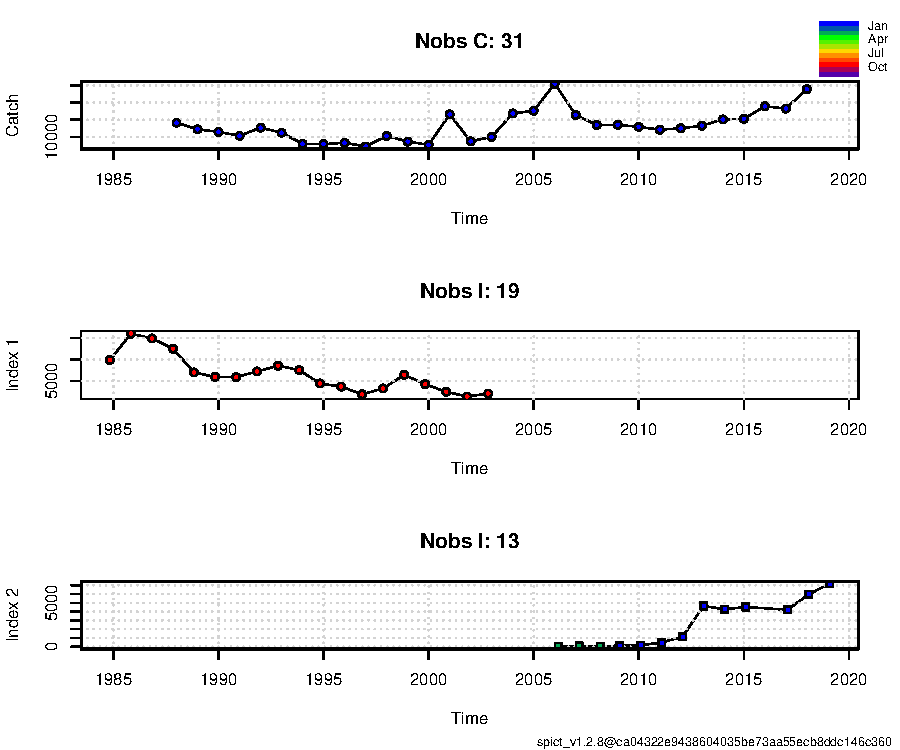
\includegraphics{aru.27.123a4_SPiCT_WD_files/figure-latex/fit_scenario1-1.pdf}

\begin{Shaded}
\begin{Highlighting}[]
\CommentTok{## Fit spict}
\NormalTok{fit_NS <-}\StringTok{ }\KeywordTok{fit.spict}\NormalTok{(inp_NS)}

\CommentTok{## Summary of the fit - in the vignette there is a line-by-line description of that summary}
\NormalTok{fit_NS}
\end{Highlighting}
\end{Shaded}

\begin{verbatim}
## Convergence: 0  MSG: relative convergence (4)
## Objective function at optimum: 57.3810526
## Euler time step (years):  1/16 or 0.0625
## Nobs C: 31,  Nobs I1: 19,  Nobs I2: 13
## 
## Priors
##      logn  ~  dnorm[log(2), 2^2]
##  logalpha  ~  dnorm[log(1), 2^2]
##   logbeta  ~  dnorm[log(1), 2^2]
## 
## Model parameter estimates w 95% CI 
##             estimate        cilow        ciupp    log.est  
##  alpha1 2.390221e+00    0.6561160 8.707540e+00  0.8713858  
##  alpha2 1.185998e+01    3.5324125 3.981958e+01  2.4731699  
##  beta   9.416977e-01    0.3601728 2.462137e+00 -0.0600710  
##  r      1.999363e-01    0.0614380 6.506482e-01 -1.6097566  
##  rc     6.376559e-01    0.0245182 1.658384e+01 -0.4499565  
##  rold   5.361626e-01    0.0090055 3.192149e+01 -0.6233178  
##  m      2.551782e+04 1202.3903015 5.415541e+05 10.1471325  
##  K      2.797479e+05 4660.6208760 1.679152e+07 12.5416442  
##  q1     1.544270e-02    0.0000792 3.010343e+00 -4.1706220  
##  q2     4.063500e-03    0.0000136 1.210055e+00 -5.5057111  
##  n      6.270977e-01    0.0459170 8.564407e+00 -0.4666529  
##  sdb    1.576217e-01    0.0512043 4.852053e-01 -1.8475574  
##  sdf    1.625876e-01    0.0768551 3.439552e-01 -1.8165384  
##  sdi1   3.767507e-01    0.2468519 5.750051e-01 -0.9761716  
##  sdi2   1.869391e+00    1.2648928 2.762781e+00  0.6256125  
##  sdc    1.531084e-01    0.0978477 2.395782e-01 -1.8766094  
##  
## Deterministic reference points (Drp)
##            estimate        cilow        ciupp   log.est  
##  Bmsyd 8.003635e+04  544.6157898 1.176209e+07 11.290236  
##  Fmsyd 3.188279e-01    0.0122591 8.291918e+00 -1.143104  
##  MSYd  2.551782e+04 1202.3903015 5.415541e+05 10.147132  
## Stochastic reference points (Srp)
##            estimate        cilow        ciupp   log.est rel.diff.Drp  
##  Bmsys 7.831263e+04  552.3440915 1.110335e+07 11.268464 -0.022010800  
##  Fmsys 3.210608e-01    0.0122407 8.421108e+00 -1.136125  0.006954625  
##  MSYs  2.514696e+04 1185.4484886 5.334435e+05 10.132492 -0.014747787  
## 
## States w 95% CI (inp$msytype: s)
##                     estimate       cilow        ciupp   log.est  
##  B_2019.08      2.203227e+05 776.4156084 6.252077e+07 12.302849  
##  F_2019.08      9.836480e-02   0.0003846 2.515559e+01 -2.319072  
##  B_2019.08/Bmsy 2.813374e+00   0.4986872 1.587182e+01  1.034385  
##  F_2019.08/Fmsy 3.063744e-01   0.0036177 2.594577e+01 -1.182947  
## 
## Predictions w 95% CI (inp$msytype: s)
##                   prediction        cilow        ciupp   log.est  
##  B_2019.08      2.203227e+05 7.764156e+02 6.252077e+07 12.302849  
##  F_2019.08      9.836480e-02 3.846000e-04 2.515559e+01 -2.319072  
##  B_2019.08/Bmsy 2.813374e+00 4.986872e-01 1.587182e+01  1.034385  
##  F_2019.08/Fmsy 3.063744e-01 3.617700e-03 2.594577e+01 -1.182947  
##  Catch_2019.08  2.110211e+04 1.295520e+04 3.437222e+04  9.957128  
##  E(B_inf)       1.727415e+05           NA           NA 12.059552
\end{verbatim}

\begin{Shaded}
\begin{Highlighting}[]
\CommentTok{## If the model converged, it reports convergence as 0}
\CommentTok{## Continue with plotting and diagnostics only if convergence was reached}
\NormalTok{converged <-}\StringTok{ }\NormalTok{fit_NS}\OperatorTok{$}\NormalTok{opt}\OperatorTok{$}\NormalTok{convergence }\OperatorTok{==}\StringTok{ }\DecValTok{0}
\ControlFlowTok{if}\NormalTok{ (converged) \{}
  \CommentTok{## Calculate the One Step Ahead (osa) residuals  }
\NormalTok{  fit_NS <-}\StringTok{ }\KeywordTok{calc.osa.resid}\NormalTok{((fit_NS))}
  
  \CommentTok{## Make a plot showing relative F, relative B, Kobe plot catch }
  \KeywordTok{par}\NormalTok{(}\DataTypeTok{mfrow =} \KeywordTok{c}\NormalTok{(}\DecValTok{2}\NormalTok{,}\DecValTok{2}\NormalTok{),  }\CommentTok{## 2x2 subplots}
      \DataTypeTok{mar =} \KeywordTok{c}\NormalTok{(}\FloatTok{4.1}\NormalTok{, }\FloatTok{4.1}\NormalTok{, }\FloatTok{0.5}\NormalTok{, }\FloatTok{0.5}\NormalTok{)) }\CommentTok{## Change default margins for the plots }
  \KeywordTok{plotspict.catch}\NormalTok{(fit_NS)}
  \KeywordTok{plotspict.ffmsy}\NormalTok{(fit_NS)}
  \KeywordTok{plotspict.bbmsy}\NormalTok{(fit_NS)}
  \KeywordTok{plotspict.fb}\NormalTok{(fit_NS)}
\NormalTok{\}}
\end{Highlighting}
\end{Shaded}

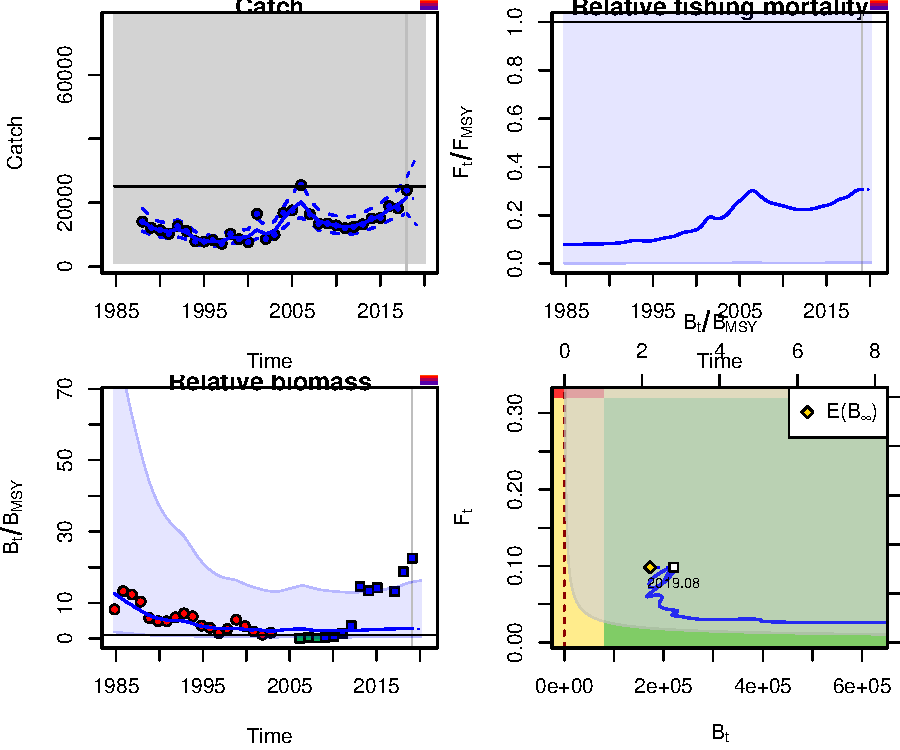
\includegraphics{aru.27.123a4_SPiCT_WD_files/figure-latex/fit_scenario1-2.pdf}

\begin{Shaded}
\begin{Highlighting}[]
\ControlFlowTok{if}\NormalTok{ (converged) \{}
  \KeywordTok{plotspict.diagnostic}\NormalTok{(fit_NS)}
\NormalTok{\}}
\end{Highlighting}
\end{Shaded}

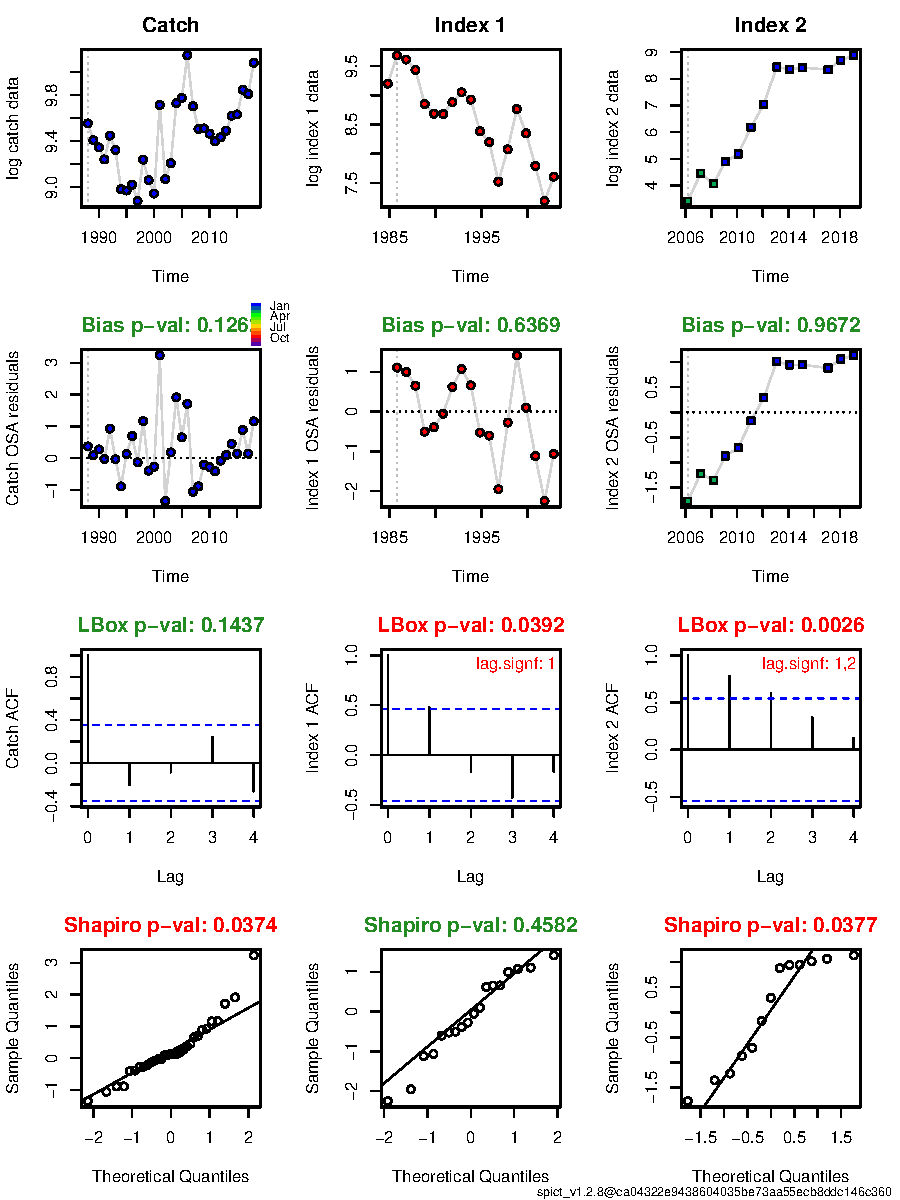
\includegraphics{aru.27.123a4_SPiCT_WD_files/figure-latex/diagnostics_scenario_1-1.pdf}

\begin{Shaded}
\begin{Highlighting}[]
  \CommentTok{## If runretro is TRUE, run and plot the retrospective analysis}
  \ControlFlowTok{if}\NormalTok{ (runretro }\OperatorTok{&}\StringTok{ }\NormalTok{converged) \{}
\NormalTok{    fit_NS <-}\StringTok{ }\KeywordTok{retro}\NormalTok{(fit_NS)}
    \KeywordTok{plotspict.retro}\NormalTok{(fit_NS)}
\NormalTok{  \}}
\end{Highlighting}
\end{Shaded}

\hypertarget{scenario-2}{%
\subsection{Scenario 2}\label{scenario-2}}

\begin{longtable}[]{@{}llll@{}}
\caption{Input data for Scenario 1}\tabularnewline
\toprule
\begin{minipage}[b]{0.21\columnwidth}\raggedright
Input data\strut
\end{minipage} & \begin{minipage}[b]{0.20\columnwidth}\raggedright
Name\strut
\end{minipage} & \begin{minipage}[b]{0.15\columnwidth}\raggedright
Range\strut
\end{minipage} & \begin{minipage}[b]{0.33\columnwidth}\raggedright
Notes\strut
\end{minipage}\tabularnewline
\midrule
\endfirsthead
\toprule
\begin{minipage}[b]{0.21\columnwidth}\raggedright
Input data\strut
\end{minipage} & \begin{minipage}[b]{0.20\columnwidth}\raggedright
Name\strut
\end{minipage} & \begin{minipage}[b]{0.15\columnwidth}\raggedright
Range\strut
\end{minipage} & \begin{minipage}[b]{0.33\columnwidth}\raggedright
Notes\strut
\end{minipage}\tabularnewline
\midrule
\endhead
\begin{minipage}[t]{0.21\columnwidth}\raggedright
Catch\strut
\end{minipage} & \begin{minipage}[t]{0.20\columnwidth}\raggedright
Total catch\strut
\end{minipage} & \begin{minipage}[t]{0.15\columnwidth}\raggedright
1988-2018\strut
\end{minipage} & \begin{minipage}[t]{0.33\columnwidth}\raggedright
\strut
\end{minipage}\tabularnewline
\begin{minipage}[t]{0.21\columnwidth}\raggedright
Biomass indices\strut
\end{minipage} & \begin{minipage}[t]{0.20\columnwidth}\raggedright
Shrimp survey\strut
\end{minipage} & \begin{minipage}[t]{0.15\columnwidth}\raggedright
1984--2002\strut
\end{minipage} & \begin{minipage}[t]{0.33\columnwidth}\raggedright
Only october period\strut
\end{minipage}\tabularnewline
\begin{minipage}[t]{0.21\columnwidth}\raggedright
Biomass indices\strut
\end{minipage} & \begin{minipage}[t]{0.20\columnwidth}\raggedright
Acoustic survey\strut
\end{minipage} & \begin{minipage}[t]{0.15\columnwidth}\raggedright
2009--2018\strut
\end{minipage} & \begin{minipage}[t]{0.33\columnwidth}\raggedright
~Matlab\strut
\end{minipage}\tabularnewline
\begin{minipage}[t]{0.21\columnwidth}\raggedright
\strut
\end{minipage} & \begin{minipage}[t]{0.20\columnwidth}\raggedright
\strut
\end{minipage} & \begin{minipage}[t]{0.15\columnwidth}\raggedright
\strut
\end{minipage} & \begin{minipage}[t]{0.33\columnwidth}\raggedright
Default priors\strut
\end{minipage}\tabularnewline
\bottomrule
\end{longtable}

\begin{Shaded}
\begin{Highlighting}[]
\CommentTok{## Choose only the years where the survey was in October }
\NormalTok{w <-}\StringTok{ }\OperatorTok{!}\KeywordTok{is.na}\NormalTok{(dat}\OperatorTok{$}\NormalTok{northsea_month) }\OperatorTok{&}\StringTok{ }\NormalTok{dat}\OperatorTok{$}\NormalTok{northsea_month }\OperatorTok{==}\StringTok{ }\DecValTok{10}
\CommentTok{## Choose only the years where the survey was in January or February }
\CommentTok{##v <- !is.na(dat$northsea_month) & dat$northsea_month %in% c(1, 2)}


\CommentTok{## Make the input list}
\NormalTok{inp_NS <-}\StringTok{ }\KeywordTok{list}\NormalTok{(}\DataTypeTok{timeC =}\NormalTok{ dat}\OperatorTok{$}\NormalTok{year,                                      }\CommentTok{## Timing of catch}
               \DataTypeTok{obsC =}\NormalTok{ dat}\OperatorTok{$}\NormalTok{catchTOT,                                   }\CommentTok{## Observed catches}
               \DataTypeTok{timeI =} \KeywordTok{list}\NormalTok{(dat}\OperatorTok{$}\NormalTok{year[w] }\OperatorTok{+}\StringTok{ }\NormalTok{dat}\OperatorTok{$}\NormalTok{northsea_month[w] }\OperatorTok{/}\StringTok{ }\DecValTok{12}\NormalTok{, }\CommentTok{## Timing of survey index}
\NormalTok{                            dat}\OperatorTok{$}\NormalTok{year}\FloatTok{+3.5}\OperatorTok{/}\DecValTok{12}\NormalTok{),}
               \DataTypeTok{obsI =} \KeywordTok{list}\NormalTok{(dat}\OperatorTok{$}\NormalTok{northsea_SA[w],                        }\CommentTok{## Observed indices}
\NormalTok{                          dat}\OperatorTok{$}\NormalTok{norwegian_seaAC),}
               \DataTypeTok{optimiser.control =} \KeywordTok{list}\NormalTok{(}\DataTypeTok{iter.max =} \FloatTok{1e5}\NormalTok{,               }\CommentTok{## Optimiser options }
                                        \DataTypeTok{eval.max =} \FloatTok{1e5}\NormalTok{),              }\CommentTok{## sometimes help converge}
               \DataTypeTok{priors =} \KeywordTok{list}\NormalTok{(                                         }\CommentTok{## List of priors (empty, i.e. default priors)}
 \DataTypeTok{logn=}\KeywordTok{c}\NormalTok{(}\KeywordTok{log}\NormalTok{(}\DecValTok{2}\NormalTok{),.}\DecValTok{5}\NormalTok{,}\DecValTok{1}\NormalTok{),}
 \DataTypeTok{logbkfrac=}\KeywordTok{c}\NormalTok{(}\KeywordTok{log}\NormalTok{(.}\DecValTok{5}\NormalTok{),}\DecValTok{1}\NormalTok{,}\DecValTok{1}\NormalTok{)}
\CommentTok{## see possible priors with list.possible.priors()}
\NormalTok{                 ))}
\CommentTok{## Check input time series, remove missing and zero observations}
\NormalTok{inp_NS <-}\StringTok{ }\KeywordTok{check.inp}\NormalTok{(inp_NS)}
\end{Highlighting}
\end{Shaded}

\begin{verbatim}
## Removing zero, negative, and NAs in  C  series    
## Removing zero, negative, and NAs in  I  series  2
\end{verbatim}

\begin{Shaded}
\begin{Highlighting}[]
\CommentTok{## Plot input data}
\KeywordTok{plotspict.data}\NormalTok{(inp_NS)}
\end{Highlighting}
\end{Shaded}

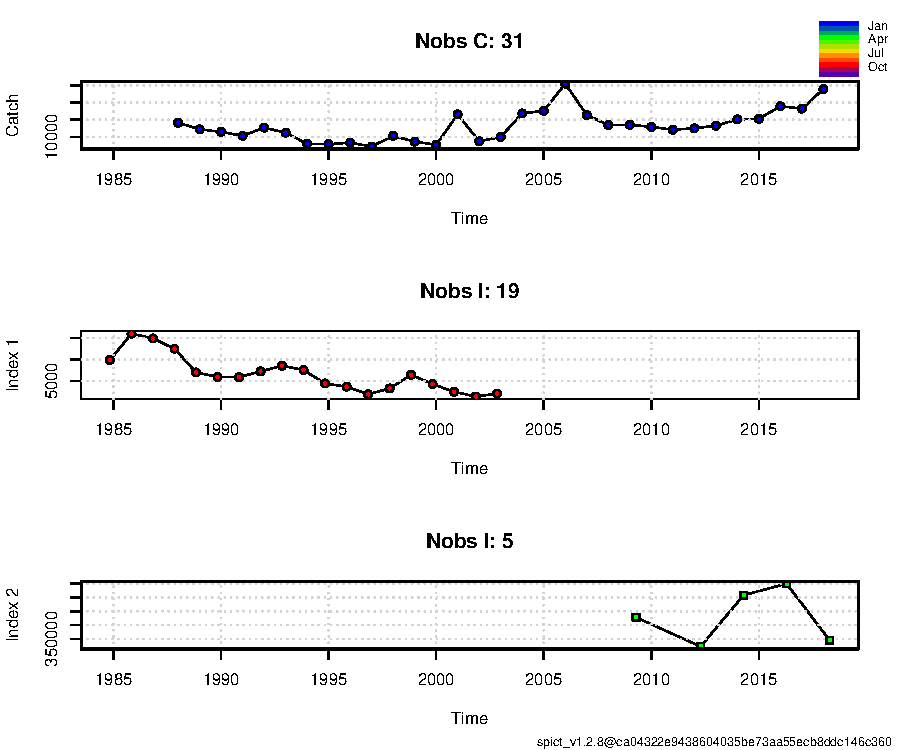
\includegraphics{aru.27.123a4_SPiCT_WD_files/figure-latex/fit_scenario2-1.pdf}

\begin{Shaded}
\begin{Highlighting}[]
\CommentTok{## Fit spict}
\NormalTok{fit_NS <-}\StringTok{ }\KeywordTok{fit.spict}\NormalTok{(inp_NS)}

\CommentTok{## Summary of the fit - in the vignette there is a line-by-line description of that summary}
\NormalTok{fit_NS}
\end{Highlighting}
\end{Shaded}

\begin{verbatim}
## Convergence: 0  MSG: relative convergence (4)
## Objective function at optimum: 28.3888908
## Euler time step (years):  1/16 or 0.0625
## Nobs C: 31,  Nobs I1: 19,  Nobs I2: 5
## 
## Priors
##       logn  ~  dnorm[log(2), 0.5^2]
##  logbkfrac  ~  dnorm[log(0.5), 1^2]
##   logalpha  ~  dnorm[log(1), 2^2]
##    logbeta  ~  dnorm[log(1), 2^2]
## 
## Model parameter estimates w 95% CI 
##             estimate        cilow        ciupp    log.est  
##  alpha1 3.110579e+00 7.699815e-01 1.256615e+01  1.1348088  
##  alpha2 1.551961e+00 3.382870e-01 7.119942e+00  0.4395195  
##  beta   1.066262e+00 4.099298e-01 2.773440e+00  0.0641595  
##  r      1.878088e-01 4.709680e-02 7.489285e-01 -1.6723309  
##  rc     2.588986e-01 4.339450e-02 1.544631e+00 -1.3513188  
##  rold   4.165855e-01 1.347390e-02 1.288001e+01 -0.8756636  
##  m      1.612555e+04 5.107054e+03 5.091651e+04  9.6881603  
##  K      2.843817e+05 3.946527e+04 2.049218e+06 12.5580725  
##  q1     1.840820e-02 1.227900e-03 2.759774e-01 -3.9949610  
##  q2     2.469988e+00 1.496627e-01 4.076394e+01  0.9042132  
##  n      1.450829e+00 5.912595e-01 3.560035e+00  0.3721351  
##  sdb    1.309317e-01 3.852300e-02 4.450098e-01 -2.0330797  
##  sdf    1.493363e-01 6.796260e-02 3.281410e-01 -1.9015548  
##  sdi1   4.072732e-01 2.634923e-01 6.295118e-01 -0.8982710  
##  sdi2   2.032009e-01 8.578800e-02 4.813095e-01 -1.5935603  
##  sdc    1.592316e-01 1.058182e-01 2.396063e-01 -1.8373952  
##  
## Deterministic reference points (Drp)
##            estimate        cilow        ciupp   log.est  
##  Bmsyd 1.245704e+05 1.438294e+04 1.078902e+06 11.732626  
##  Fmsyd 1.294493e-01 2.169730e-02 7.723154e-01 -2.044466  
##  MSYd  1.612555e+04 5.107054e+03 5.091651e+04  9.688160  
## Stochastic reference points (Srp)
##            estimate        cilow        ciupp   log.est rel.diff.Drp  
##  Bmsys 1.200232e+05 1.417972e+04 1.015927e+06 11.695440  -0.03788633  
##  Fmsys 1.275264e-01 2.049930e-02 7.933447e-01 -2.059432  -0.01507846  
##  MSYs  1.529738e+04 4.830986e+03 4.843934e+04  9.635437  -0.05413822  
## 
## States w 95% CI (inp$msytype: s)
##                     estimate        cilow        ciupp    log.est  
##  B_2018.27      1.704629e+05 9476.1521410 3.066391e+06 12.0462727  
##  F_2018.27      1.197088e-01    0.0067759 2.114883e+00 -2.1226934  
##  B_2018.27/Bmsy 1.420250e+00    0.4788558 4.212352e+00  0.3508327  
##  F_2018.27/Fmsy 9.386979e-01    0.1126937 7.819019e+00 -0.0632615  
## 
## Predictions w 95% CI (inp$msytype: s)
##                   prediction        cilow        ciupp    log.est  
##  B_2019.02      1.684139e+05 8.707537e+03 3.257320e+06 12.0341797  
##  F_2019.02      1.230908e-01 6.825200e-03 2.219921e+00 -2.0948329  
##  B_2019.02/Bmsy 1.403178e+00 4.395614e-01 4.479258e+00  0.3387398  
##  F_2019.02/Fmsy 9.652182e-01 1.128026e-01 8.259088e+00 -0.0354011  
##  Catch_2019.00  2.037854e+04 1.329067e+04 3.124637e+04  9.9222378  
##  E(B_inf)       1.165644e+05           NA           NA 11.6661995
\end{verbatim}

\begin{Shaded}
\begin{Highlighting}[]
\CommentTok{## If the model converged, it reports convergence as 0}
\CommentTok{## Continue with plotting and diagnostics only if convergence was reached}
\NormalTok{converged <-}\StringTok{ }\NormalTok{fit_NS}\OperatorTok{$}\NormalTok{opt}\OperatorTok{$}\NormalTok{convergence }\OperatorTok{==}\StringTok{ }\DecValTok{0}
\ControlFlowTok{if}\NormalTok{ (converged) \{}
  \CommentTok{## Calculate the One Step Ahead (osa) residuals  }
\NormalTok{  fit_NS <-}\StringTok{ }\KeywordTok{calc.osa.resid}\NormalTok{((fit_NS))}
  
  \CommentTok{## Make a plot showing relative F, relative B, Kobe plot catch }
  \KeywordTok{par}\NormalTok{(}\DataTypeTok{mfrow =} \KeywordTok{c}\NormalTok{(}\DecValTok{2}\NormalTok{,}\DecValTok{2}\NormalTok{),  }\CommentTok{## 2x2 subplots}
      \DataTypeTok{mar =} \KeywordTok{c}\NormalTok{(}\FloatTok{4.1}\NormalTok{, }\FloatTok{4.1}\NormalTok{, }\FloatTok{0.5}\NormalTok{, }\FloatTok{0.5}\NormalTok{)) }\CommentTok{## Change default margins for the plots }
  \KeywordTok{plotspict.catch}\NormalTok{(fit_NS)}
  \KeywordTok{plotspict.ffmsy}\NormalTok{(fit_NS)}
  \KeywordTok{plotspict.bbmsy}\NormalTok{(fit_NS)}
  \KeywordTok{plotspict.fb}\NormalTok{(fit_NS)}
\NormalTok{\}}
\end{Highlighting}
\end{Shaded}

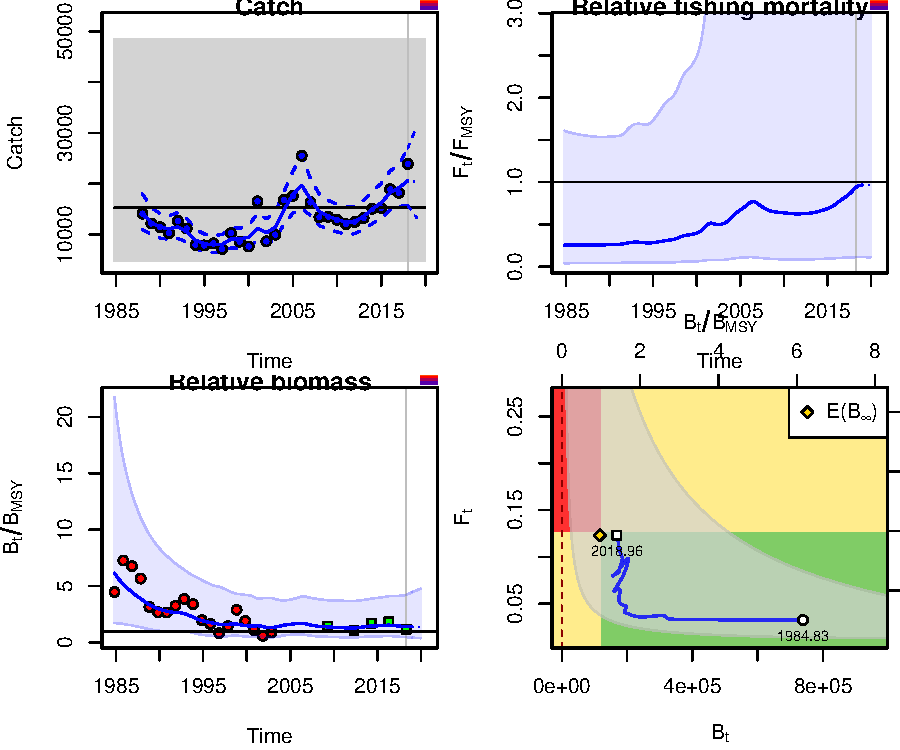
\includegraphics{aru.27.123a4_SPiCT_WD_files/figure-latex/fit_scenario2-2.pdf}

\begin{Shaded}
\begin{Highlighting}[]
\ControlFlowTok{if}\NormalTok{ (converged) \{}
  \KeywordTok{plotspict.diagnostic}\NormalTok{(fit_NS)}
  \KeywordTok{plotspict.production}\NormalTok{(fit_NS)}
\NormalTok{\}}
\end{Highlighting}
\end{Shaded}

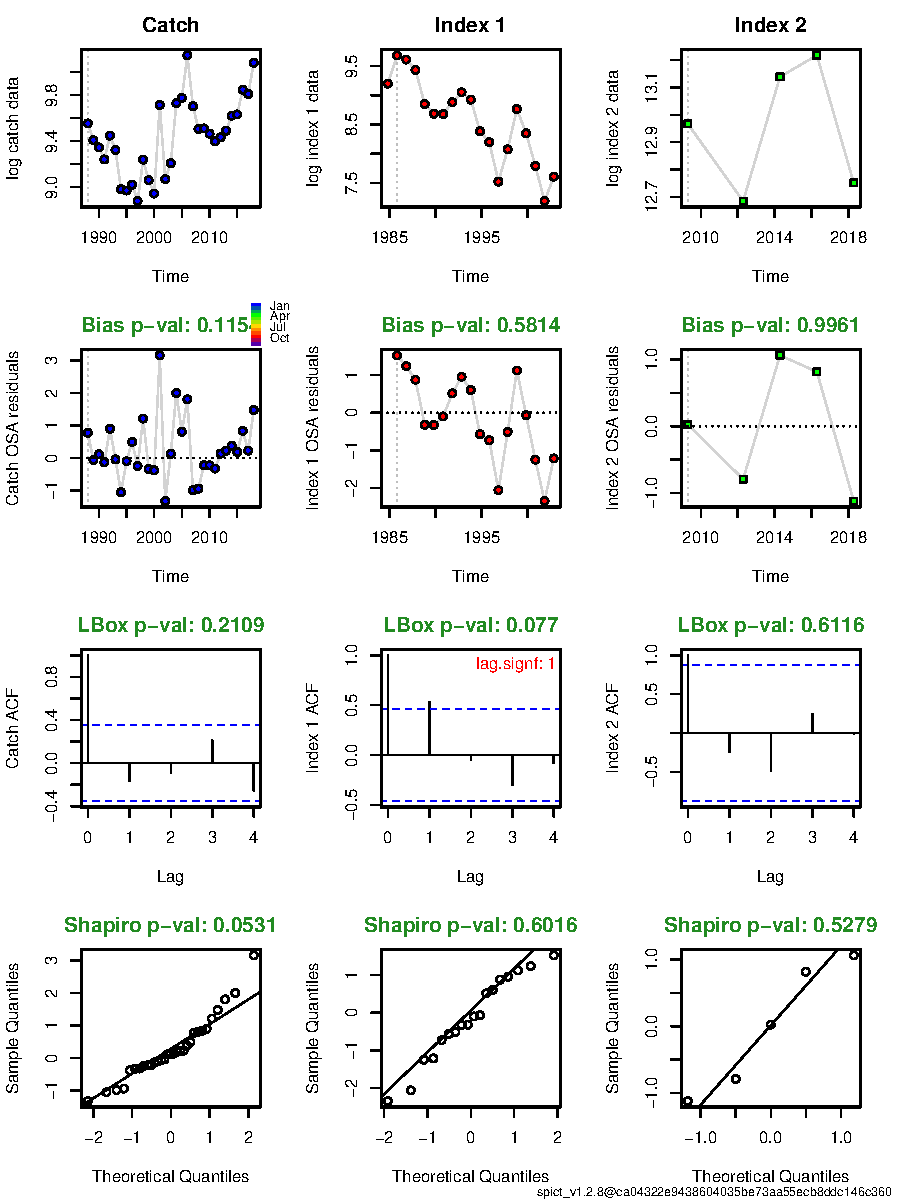
\includegraphics{aru.27.123a4_SPiCT_WD_files/figure-latex/diagnostics_scenario_2-1.pdf}
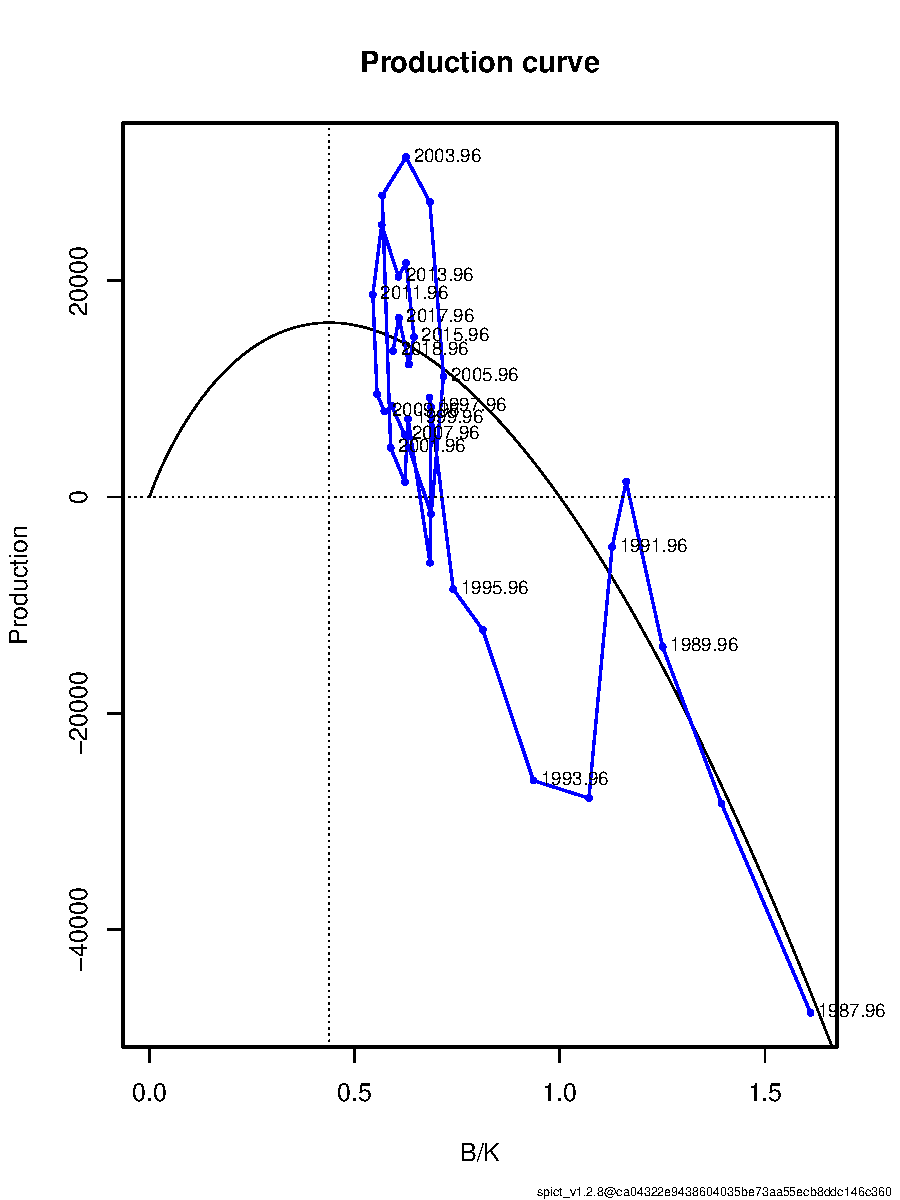
\includegraphics{aru.27.123a4_SPiCT_WD_files/figure-latex/diagnostics_scenario_2-2.pdf}

\begin{Shaded}
\begin{Highlighting}[]
  \CommentTok{## If runretro is TRUE, run and plot the retrospective analysis}
  \ControlFlowTok{if}\NormalTok{ (runretro }\OperatorTok{&}\StringTok{ }\NormalTok{converged) \{}
\NormalTok{    fit_NS <-}\StringTok{ }\KeywordTok{retro}\NormalTok{(fit_NS)}
    \KeywordTok{plotspict.retro}\NormalTok{(fit_NS)}
\NormalTok{  \}}
\end{Highlighting}
\end{Shaded}

\hypertarget{scenario-3}{%
\subsection{Scenario 3}\label{scenario-3}}

\begin{longtable}[]{@{}llll@{}}
\caption{Input data for Scenario 3}\tabularnewline
\toprule
\begin{minipage}[b]{0.21\columnwidth}\raggedright
Input data\strut
\end{minipage} & \begin{minipage}[b]{0.20\columnwidth}\raggedright
Name\strut
\end{minipage} & \begin{minipage}[b]{0.15\columnwidth}\raggedright
Range\strut
\end{minipage} & \begin{minipage}[b]{0.33\columnwidth}\raggedright
Notes\strut
\end{minipage}\tabularnewline
\midrule
\endfirsthead
\toprule
\begin{minipage}[b]{0.21\columnwidth}\raggedright
Input data\strut
\end{minipage} & \begin{minipage}[b]{0.20\columnwidth}\raggedright
Name\strut
\end{minipage} & \begin{minipage}[b]{0.15\columnwidth}\raggedright
Range\strut
\end{minipage} & \begin{minipage}[b]{0.33\columnwidth}\raggedright
Notes\strut
\end{minipage}\tabularnewline
\midrule
\endhead
\begin{minipage}[t]{0.21\columnwidth}\raggedright
Catch\strut
\end{minipage} & \begin{minipage}[t]{0.20\columnwidth}\raggedright
Total catch\strut
\end{minipage} & \begin{minipage}[t]{0.15\columnwidth}\raggedright
1988-2018\strut
\end{minipage} & \begin{minipage}[t]{0.33\columnwidth}\raggedright
\strut
\end{minipage}\tabularnewline
\begin{minipage}[t]{0.21\columnwidth}\raggedright
Biomass indices\strut
\end{minipage} & \begin{minipage}[t]{0.20\columnwidth}\raggedright
Acoustic survey\strut
\end{minipage} & \begin{minipage}[t]{0.15\columnwidth}\raggedright
2009--2018\strut
\end{minipage} & \begin{minipage}[t]{0.33\columnwidth}\raggedright
~Matlab\strut
\end{minipage}\tabularnewline
\begin{minipage}[t]{0.21\columnwidth}\raggedright
Biomass indices\strut
\end{minipage} & \begin{minipage}[t]{0.20\columnwidth}\raggedright
Acoustic survey\strut
\end{minipage} & \begin{minipage}[t]{0.15\columnwidth}\raggedright
1990-1993\strut
\end{minipage} & \begin{minipage}[t]{0.33\columnwidth}\raggedright
~Monstad\strut
\end{minipage}\tabularnewline
\begin{minipage}[t]{0.21\columnwidth}\raggedright
\strut
\end{minipage} & \begin{minipage}[t]{0.20\columnwidth}\raggedright
\strut
\end{minipage} & \begin{minipage}[t]{0.15\columnwidth}\raggedright
\strut
\end{minipage} & \begin{minipage}[t]{0.33\columnwidth}\raggedright
Default priors\strut
\end{minipage}\tabularnewline
\bottomrule
\end{longtable}

\begin{Shaded}
\begin{Highlighting}[]
\CommentTok{## Choose only the years where the survey was in October }
\NormalTok{w <-}\StringTok{ }\OperatorTok{!}\KeywordTok{is.na}\NormalTok{(dat}\OperatorTok{$}\NormalTok{northsea_month) }\OperatorTok{&}\StringTok{ }\NormalTok{dat}\OperatorTok{$}\NormalTok{northsea_month }\OperatorTok{==}\StringTok{ }\DecValTok{10}
\CommentTok{## Choose only the years where the survey was in January or February }
\CommentTok{##v <- !is.na(dat$northsea_month) & dat$northsea_month %in% c(1, 2)}


\CommentTok{## Make the input list}
\NormalTok{inp_NS <-}\StringTok{ }\KeywordTok{list}\NormalTok{(}\DataTypeTok{timeC =}\NormalTok{ dat}\OperatorTok{$}\NormalTok{year,                                      }\CommentTok{## Timing of catch}
               \DataTypeTok{obsC =}\NormalTok{ dat}\OperatorTok{$}\NormalTok{catchTOT,                                   }\CommentTok{## Observed catches}
               \DataTypeTok{timeI =} \KeywordTok{list}\NormalTok{(dat}\OperatorTok{$}\NormalTok{year}\FloatTok{+3.5}\OperatorTok{/}\DecValTok{12}\NormalTok{,dat}\OperatorTok{$}\NormalTok{year}\OperatorTok{+}\DecValTok{3}\OperatorTok{/}\DecValTok{12}\NormalTok{),}\CommentTok{## Timing of survey index}
               \DataTypeTok{obsI =} \KeywordTok{list}\NormalTok{(dat}\OperatorTok{$}\NormalTok{norwegian_seaAC,dat}\OperatorTok{$}\NormalTok{Norwegian_seaAC_Monstad), }\CommentTok{## Observed indices}
               \DataTypeTok{optimiser.control =} \KeywordTok{list}\NormalTok{(}\DataTypeTok{iter.max =} \FloatTok{1e3}\NormalTok{,               }\CommentTok{## Optimiser options }
                                        \DataTypeTok{eval.max =} \FloatTok{1e3}\NormalTok{),              }\CommentTok{## sometimes help converge}
               \DataTypeTok{priors =} \KeywordTok{list}\NormalTok{(                                         }\CommentTok{## List of priors (empty, i.e. default priors)}
 \CommentTok{#logn=c(log(2),.5,1),}
 \CommentTok{#logbkfrac=c(log(.5),1,1)}
\CommentTok{## see possible priors with list.possible.priors()}
\NormalTok{                 ))}
\CommentTok{## Check input time series, remove missing and zero observations}
\NormalTok{inp_NS <-}\StringTok{ }\KeywordTok{check.inp}\NormalTok{(inp_NS)}
\end{Highlighting}
\end{Shaded}

\begin{verbatim}
## Removing zero, negative, and NAs in  C  series    
## Removing zero, negative, and NAs in  I  series  1  
## Removing zero, negative, and NAs in  I  series  2
\end{verbatim}

\begin{Shaded}
\begin{Highlighting}[]
\CommentTok{## Plot input data}
\KeywordTok{plotspict.data}\NormalTok{(inp_NS)}
\end{Highlighting}
\end{Shaded}

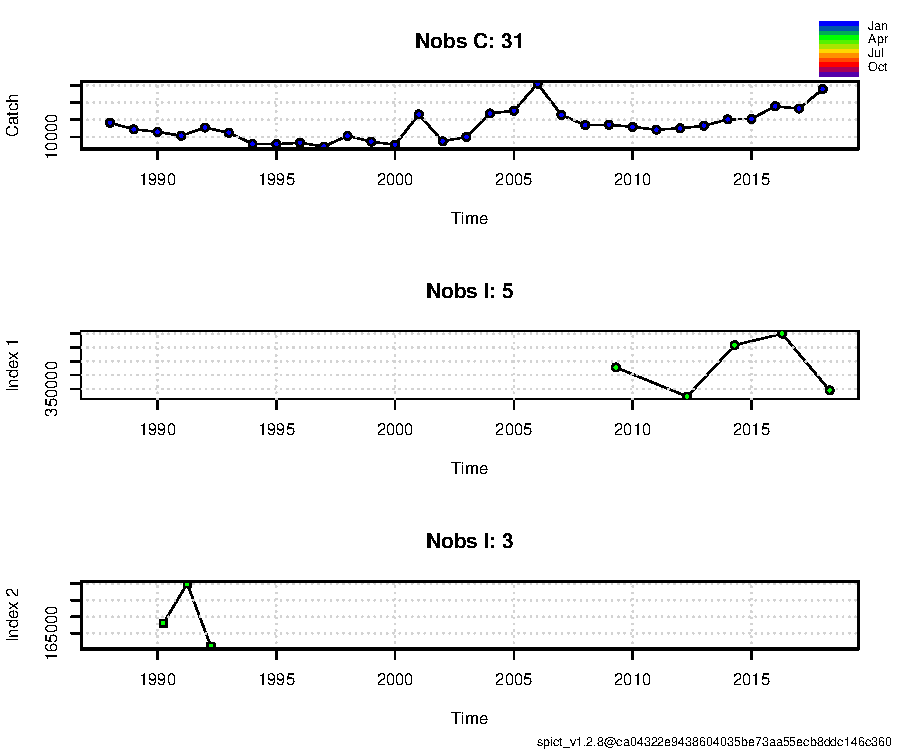
\includegraphics{aru.27.123a4_SPiCT_WD_files/figure-latex/fit_scenario3-1.pdf}

\begin{Shaded}
\begin{Highlighting}[]
\CommentTok{## Fit spict}
\NormalTok{fit_NS <-}\StringTok{ }\KeywordTok{fit.spict}\NormalTok{(inp_NS)}

\CommentTok{## Summary of the fit - in the vignette there is a line-by-line description of that summary}
\NormalTok{fit_NS}
\end{Highlighting}
\end{Shaded}

\begin{verbatim}
## Convergence: 0  MSG: relative convergence (4)
## Objective function at optimum: 14.3407429
## Euler time step (years):  1/16 or 0.0625
## Nobs C: 31,  Nobs I1: 5,  Nobs I2: 3
## 
## Priors
##      logn  ~  dnorm[log(2), 2^2]
##  logalpha  ~  dnorm[log(1), 2^2]
##   logbeta  ~  dnorm[log(1), 2^2]
## 
## Model parameter estimates w 95% CI 
##             estimate        cilow        ciupp    log.est  
##  alpha1 5.756276e+00 8.811767e-01 3.760281e+01  1.7502908  
##  alpha2 1.431561e+00 1.678045e-01 1.221284e+01  0.3587658  
##  beta   9.080295e-01 3.292256e-01 2.504415e+00 -0.0964785  
##  r      4.896562e-01 4.112190e-02 5.830555e+00 -0.7140517  
##  rc     4.770468e-01 1.828155e-01 1.244827e+00 -0.7401407  
##  rold   4.650705e-01 1.956400e-02 1.105556e+01 -0.7655663  
##  m      1.595670e+04 1.147293e+04 2.219278e+04  9.6776338  
##  K      1.324612e+05 4.637432e+04 3.783552e+05 11.7940448  
##  q1     5.779729e+00 1.367156e+00 2.443413e+01  1.7543568  
##  q2     5.761715e+00 1.062269e+00 3.125138e+01  1.7512351  
##  n      2.052865e+00 1.303502e-01 3.233023e+01  0.7192361  
##  sdb    3.434090e-02 5.769200e-03 2.044128e-01 -3.3714171  
##  sdf    1.768985e-01 8.492990e-02 3.684577e-01 -1.7321790  
##  sdi1   1.976759e-01 1.014676e-01 3.851061e-01 -1.6211263  
##  sdi2   4.916120e-02 1.558680e-02 1.550557e-01 -3.0126513  
##  sdc    1.606291e-01 1.055958e-01 2.443441e-01 -1.8286574  
##  
## Deterministic reference points (Drp)
##            estimate        cilow        ciupp   log.est  
##  Bmsyd 6.689782e+04 2.193877e+04 2.039913e+05 11.110922  
##  Fmsyd 2.385234e-01 9.140780e-02 6.224133e-01 -1.433288  
##  MSYd  1.595670e+04 1.147293e+04 2.219278e+04  9.677634  
## Stochastic reference points (Srp)
##            estimate        cilow        ciupp   log.est rel.diff.Drp  
##  Bmsys 6.679055e+04 2.190420e+04 2.036585e+05 11.109317 -0.001606076  
##  Fmsys 2.382187e-01 9.101280e-02 6.235185e-01 -1.434566 -0.001279081  
##  MSYs  1.591072e+04 1.148177e+04 2.204808e+04  9.674749 -0.002889347  
## 
## States w 95% CI (inp$msytype: s)
##                     estimate        cilow        ciupp    log.est  
##  B_2018.25      7.035036e+04 1.489201e+04 3.323375e+05 11.1612432  
##  F_2018.25      2.935164e-01 6.110920e-02 1.409802e+00 -1.2258218  
##  B_2018.25/Bmsy 1.053298e+00 4.969773e-01 2.232369e+00  0.0519263  
##  F_2018.25/Fmsy 1.232130e+00 4.324268e-01 3.510755e+00  0.2087444  
## 
## Predictions w 95% CI (inp$msytype: s)
##                   prediction        cilow        ciupp    log.est  
##  B_2019.00      6.682726e+04 1.260149e+04 3.543933e+05 11.1098663  
##  F_2019.00      3.064146e-01 6.034140e-02 1.555978e+00 -1.1828162  
##  B_2019.00/Bmsy 1.000550e+00 4.288084e-01 2.334608e+00  0.0005494  
##  F_2019.00/Fmsy 1.286274e+00 4.273219e-01 3.871792e+00  0.2517500  
##  Catch_2019.00  1.987688e+04 1.371934e+04 2.879807e+04  9.8973127  
##  E(B_inf)       4.723742e+04           NA           NA 10.7629416
\end{verbatim}

\begin{Shaded}
\begin{Highlighting}[]
\CommentTok{## If the model converged, it reports convergence as 0}
\CommentTok{## Continue with plotting and diagnostics only if convergence was reached}
\NormalTok{converged <-}\StringTok{ }\NormalTok{fit_NS}\OperatorTok{$}\NormalTok{opt}\OperatorTok{$}\NormalTok{convergence }\OperatorTok{==}\StringTok{ }\DecValTok{0}
\ControlFlowTok{if}\NormalTok{ (converged) \{}
  \CommentTok{## Calculate the One Step Ahead (osa) residuals  }
\NormalTok{  fit_NS <-}\StringTok{ }\KeywordTok{calc.osa.resid}\NormalTok{((fit_NS))}
  
  \CommentTok{## Make a plot showing relative F, relative B, Kobe plot catch }
  \KeywordTok{par}\NormalTok{(}\DataTypeTok{mfrow =} \KeywordTok{c}\NormalTok{(}\DecValTok{2}\NormalTok{,}\DecValTok{2}\NormalTok{),  }\CommentTok{## 2x2 subplots}
      \DataTypeTok{mar =} \KeywordTok{c}\NormalTok{(}\FloatTok{4.1}\NormalTok{, }\FloatTok{4.1}\NormalTok{, }\FloatTok{0.5}\NormalTok{, }\FloatTok{0.5}\NormalTok{)) }\CommentTok{## Change default margins for the plots }
  \KeywordTok{plotspict.catch}\NormalTok{(fit_NS)}
  \KeywordTok{plotspict.ffmsy}\NormalTok{(fit_NS)}
  \KeywordTok{plotspict.bbmsy}\NormalTok{(fit_NS)}
  \KeywordTok{plotspict.fb}\NormalTok{(fit_NS)}
\NormalTok{\}}
\end{Highlighting}
\end{Shaded}

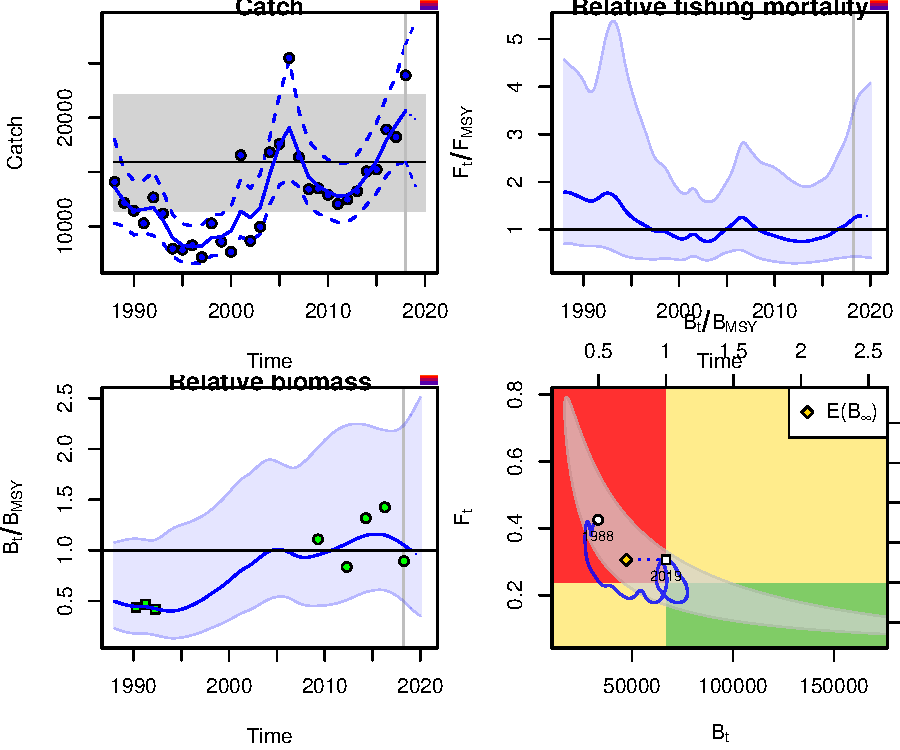
\includegraphics{aru.27.123a4_SPiCT_WD_files/figure-latex/fit_scenario3-2.pdf}

\begin{Shaded}
\begin{Highlighting}[]
\ControlFlowTok{if}\NormalTok{ (converged) \{}
  \KeywordTok{plotspict.diagnostic}\NormalTok{(fit_NS)}
  \KeywordTok{plotspict.production}\NormalTok{(fit_NS)}
\NormalTok{\}}
\end{Highlighting}
\end{Shaded}

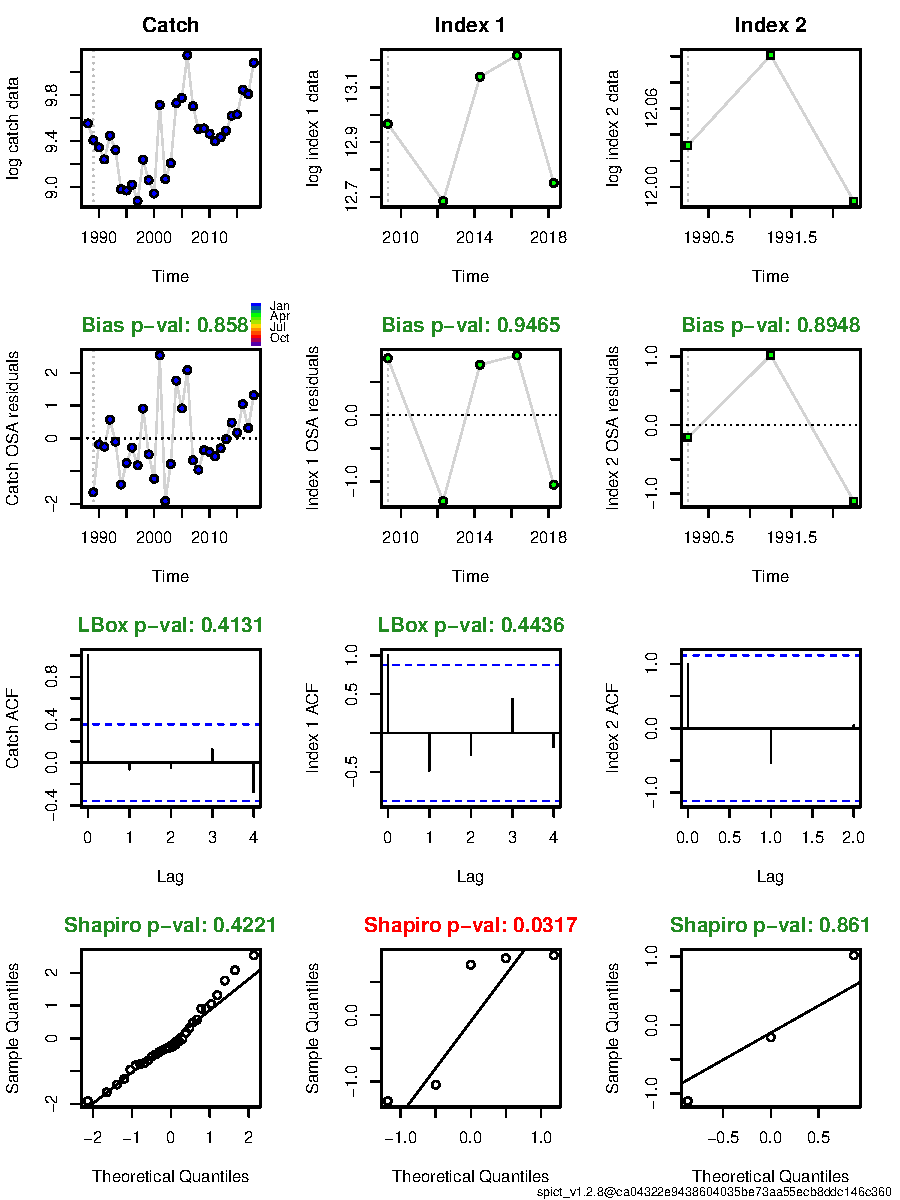
\includegraphics{aru.27.123a4_SPiCT_WD_files/figure-latex/diagnostics_scenario_3-1.pdf}
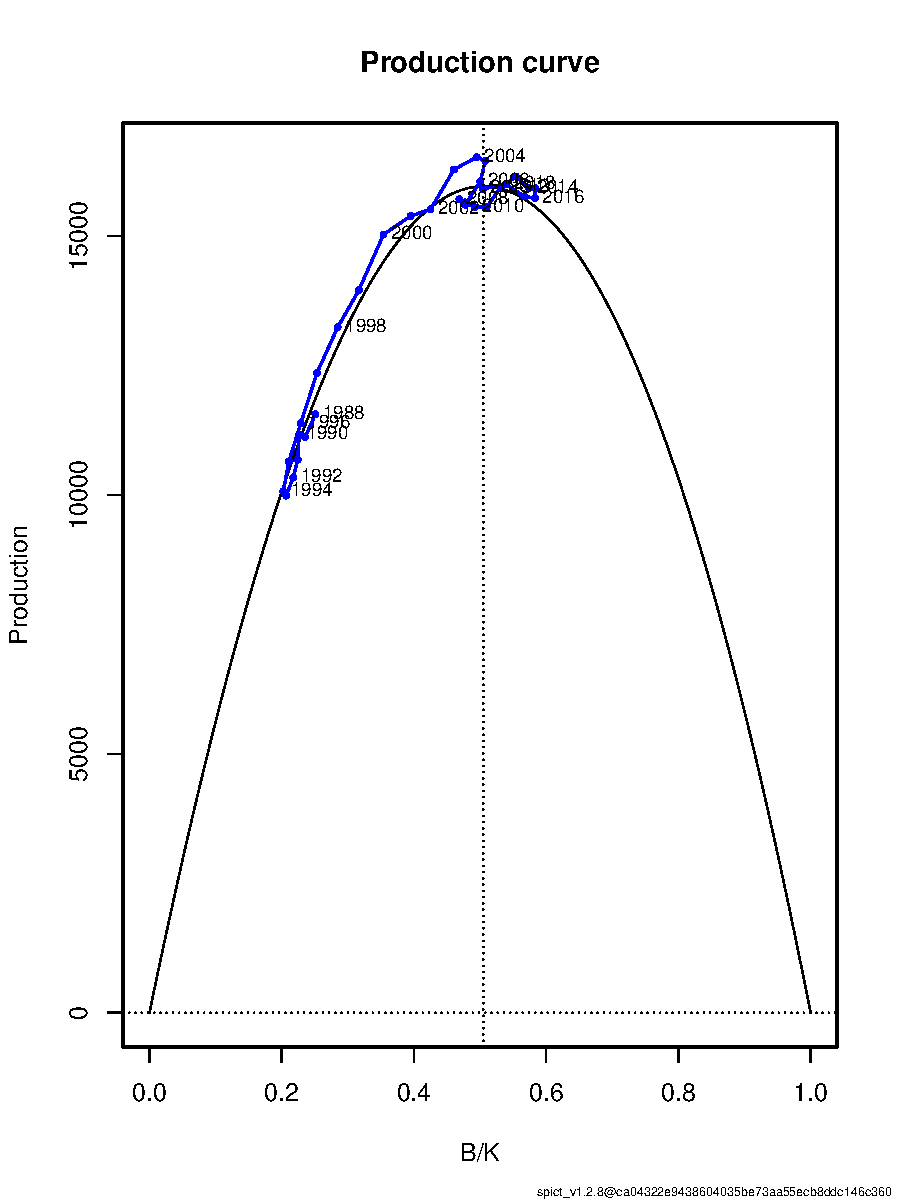
\includegraphics{aru.27.123a4_SPiCT_WD_files/figure-latex/diagnostics_scenario_3-2.pdf}

\begin{Shaded}
\begin{Highlighting}[]
  \CommentTok{## If runretro is TRUE, run and plot the retrospective analysis}
  \CommentTok{#runretro=TRUE}
\ControlFlowTok{if}\NormalTok{ (runretro }\OperatorTok{&}\StringTok{ }\NormalTok{converged) \{}
\NormalTok{    fit_NS <-}\StringTok{ }\KeywordTok{retro}\NormalTok{(fit_NS)}
    \KeywordTok{plotspict.retro}\NormalTok{(fit_NS)}
\NormalTok{  \}}
\end{Highlighting}
\end{Shaded}

\hypertarget{scenario-4}{%
\subsection{Scenario 4}\label{scenario-4}}

\begin{longtable}[]{@{}llll@{}}
\caption{Input data for Scenario 4}\tabularnewline
\toprule
\begin{minipage}[b]{0.21\columnwidth}\raggedright
Input data\strut
\end{minipage} & \begin{minipage}[b]{0.20\columnwidth}\raggedright
Name\strut
\end{minipage} & \begin{minipage}[b]{0.15\columnwidth}\raggedright
Range\strut
\end{minipage} & \begin{minipage}[b]{0.33\columnwidth}\raggedright
Notes\strut
\end{minipage}\tabularnewline
\midrule
\endfirsthead
\toprule
\begin{minipage}[b]{0.21\columnwidth}\raggedright
Input data\strut
\end{minipage} & \begin{minipage}[b]{0.20\columnwidth}\raggedright
Name\strut
\end{minipage} & \begin{minipage}[b]{0.15\columnwidth}\raggedright
Range\strut
\end{minipage} & \begin{minipage}[b]{0.33\columnwidth}\raggedright
Notes\strut
\end{minipage}\tabularnewline
\midrule
\endhead
\begin{minipage}[t]{0.21\columnwidth}\raggedright
Catch\strut
\end{minipage} & \begin{minipage}[t]{0.20\columnwidth}\raggedright
Total catch\strut
\end{minipage} & \begin{minipage}[t]{0.15\columnwidth}\raggedright
1988-2018\strut
\end{minipage} & \begin{minipage}[t]{0.33\columnwidth}\raggedright
\strut
\end{minipage}\tabularnewline
\begin{minipage}[t]{0.21\columnwidth}\raggedright
Biomass indices\strut
\end{minipage} & \begin{minipage}[t]{0.20\columnwidth}\raggedright
Acoustic survey\strut
\end{minipage} & \begin{minipage}[t]{0.15\columnwidth}\raggedright
2012--2018\strut
\end{minipage} & \begin{minipage}[t]{0.33\columnwidth}\raggedright
~StoX\strut
\end{minipage}\tabularnewline
\begin{minipage}[t]{0.21\columnwidth}\raggedright
Biomass indices\strut
\end{minipage} & \begin{minipage}[t]{0.20\columnwidth}\raggedright
Acoustic survey\strut
\end{minipage} & \begin{minipage}[t]{0.15\columnwidth}\raggedright
1990-1993\strut
\end{minipage} & \begin{minipage}[t]{0.33\columnwidth}\raggedright
~Monstad\strut
\end{minipage}\tabularnewline
\begin{minipage}[t]{0.21\columnwidth}\raggedright
\strut
\end{minipage} & \begin{minipage}[t]{0.20\columnwidth}\raggedright
\strut
\end{minipage} & \begin{minipage}[t]{0.15\columnwidth}\raggedright
\strut
\end{minipage} & \begin{minipage}[t]{0.33\columnwidth}\raggedright
Default priors\strut
\end{minipage}\tabularnewline
\bottomrule
\end{longtable}

\begin{Shaded}
\begin{Highlighting}[]
\CommentTok{## Choose only the years where the survey was in October }
\NormalTok{w <-}\StringTok{ }\OperatorTok{!}\KeywordTok{is.na}\NormalTok{(dat}\OperatorTok{$}\NormalTok{northsea_month) }\OperatorTok{&}\StringTok{ }\NormalTok{dat}\OperatorTok{$}\NormalTok{northsea_month }\OperatorTok{==}\StringTok{ }\DecValTok{10}
\NormalTok{w[}\DecValTok{1}\OperatorTok{:}\DecValTok{4}\NormalTok{]<-}\OtherTok{FALSE}
\CommentTok{## Choose only the years where the survey was in January or February }
\CommentTok{##v <- !is.na(dat$northsea_month) & dat$northsea_month %in% c(1, 2)}


\CommentTok{## Make the input list}
\NormalTok{inp_NS <-}\StringTok{ }\KeywordTok{list}\NormalTok{(}\DataTypeTok{timeC =}\NormalTok{ dat}\OperatorTok{$}\NormalTok{year,                                      }\CommentTok{## Timing of catch}
               \DataTypeTok{obsC =}\NormalTok{ dat}\OperatorTok{$}\NormalTok{catchTOT,                                   }\CommentTok{## Observed catches}
               \DataTypeTok{timeI =} \KeywordTok{list}\NormalTok{(dat}\OperatorTok{$}\NormalTok{year}\FloatTok{+3.5}\OperatorTok{/}\DecValTok{12}\NormalTok{, dat}\OperatorTok{$}\NormalTok{year}\OperatorTok{+}\DecValTok{3}\OperatorTok{/}\DecValTok{12}\NormalTok{),}
               \DataTypeTok{obsI =} \KeywordTok{list}\NormalTok{(dat}\OperatorTok{$}\NormalTok{norwegian_seaAC,dat}\OperatorTok{$}\NormalTok{Norwegian_seaAC_Monstad),}
               \DataTypeTok{optimiser.control =} \KeywordTok{list}\NormalTok{(}\DataTypeTok{iter.max =} \FloatTok{1e3}\NormalTok{,               }\CommentTok{## Optimiser options }
                                        \DataTypeTok{eval.max =} \FloatTok{1e3}\NormalTok{),              }\CommentTok{## sometimes help converge}
               \DataTypeTok{priors =} \KeywordTok{list}\NormalTok{(                                         }\CommentTok{## List of priors (empty, i.e. default priors)}
 \DataTypeTok{logn=}\KeywordTok{c}\NormalTok{(}\KeywordTok{log}\NormalTok{(}\DecValTok{2}\NormalTok{),.}\DecValTok{5}\NormalTok{,}\DecValTok{1}\NormalTok{)}
 \CommentTok{#logbkfrac=c(log(.5),1,1)}
\CommentTok{## see possible priors with list.possible.priors()}
\NormalTok{                 ))}
\CommentTok{## Check input time series, remove missing and zero observations}
\NormalTok{inp_NS <-}\StringTok{ }\KeywordTok{check.inp}\NormalTok{(inp_NS)}
\end{Highlighting}
\end{Shaded}

\begin{verbatim}
## Removing zero, negative, and NAs in  C  series    
## Removing zero, negative, and NAs in  I  series  1  
## Removing zero, negative, and NAs in  I  series  2
\end{verbatim}

\begin{Shaded}
\begin{Highlighting}[]
\CommentTok{## Plot input data}
\KeywordTok{plotspict.data}\NormalTok{(inp_NS)}
\end{Highlighting}
\end{Shaded}

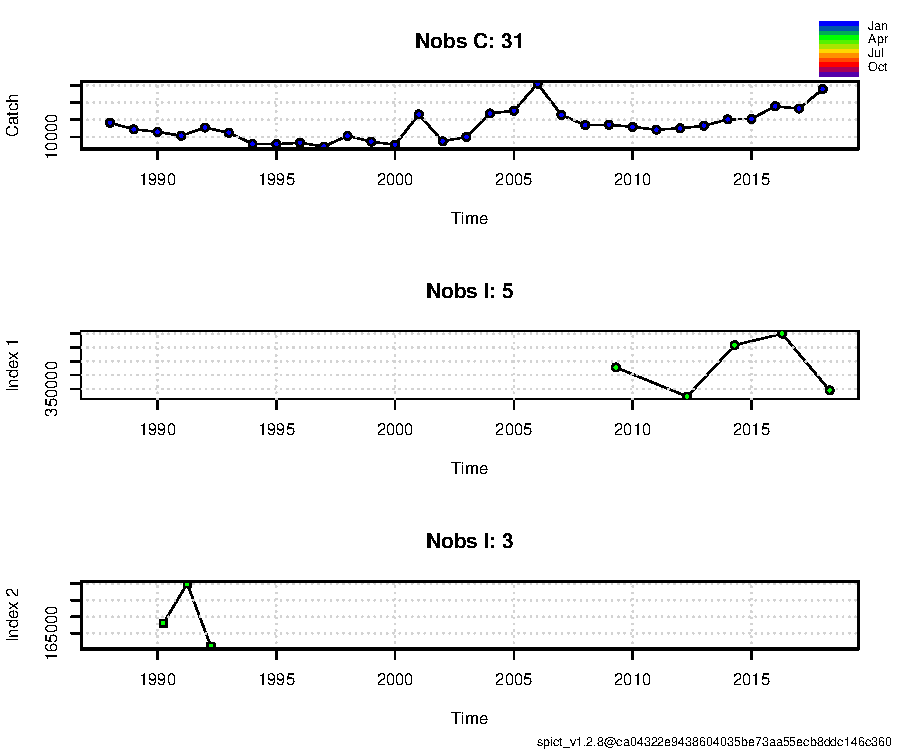
\includegraphics{aru.27.123a4_SPiCT_WD_files/figure-latex/fit_scenario4-1.pdf}

\begin{Shaded}
\begin{Highlighting}[]
\CommentTok{## Fit spict}
\NormalTok{fit_AC <-}\StringTok{ }\KeywordTok{fit.spict}\NormalTok{(inp_NS)}

\CommentTok{## Summary of the fit - in the vignette there is a line-by-line description of that summary}
\NormalTok{fit_AC}
\end{Highlighting}
\end{Shaded}

\begin{verbatim}
## Convergence: 0  MSG: relative convergence (4)
## Objective function at optimum: 12.9546007
## Euler time step (years):  1/16 or 0.0625
## Nobs C: 31,  Nobs I1: 5,  Nobs I2: 3
## 
## Priors
##      logn  ~  dnorm[log(2), 0.5^2]
##  logalpha  ~  dnorm[log(1), 2^2]
##   logbeta  ~  dnorm[log(1), 2^2]
## 
## Model parameter estimates w 95% CI 
##             estimate        cilow        ciupp    log.est  
##  alpha1 5.735290e+00 9.167939e-01 3.587889e+01  1.7466383  
##  alpha2 1.426235e+00 1.733854e-01 1.173193e+01  0.3550379  
##  beta   9.053337e-01 3.469476e-01 2.362401e+00 -0.0994517  
##  r      4.802329e-01 1.475322e-01 1.563209e+00 -0.7334841  
##  rc     4.787391e-01 1.996902e-01 1.147734e+00 -0.7365994  
##  rold   4.772546e-01 1.191177e-01 1.912159e+00 -0.7397051  
##  m      1.593563e+04 1.194744e+04 2.125514e+04  9.6763129  
##  K      1.329867e+05 5.068315e+04 3.489414e+05 11.7980040  
##  q1     5.828785e+00 1.983238e+00 1.713094e+01  1.7628085  
##  q2     5.828383e+00 1.963658e+00 1.729937e+01  1.7627397  
##  n      2.006240e+00 7.762974e-01 5.184869e+00  0.6962625  
##  sdb    3.446170e-02 6.040500e-03 1.966066e-01 -3.3679081  
##  sdf    1.772791e-01 8.862120e-02 3.546316e-01 -1.7300302  
##  sdi1   1.976476e-01 1.013611e-01 3.854000e-01 -1.6212698  
##  sdi2   4.915040e-02 1.551090e-02 1.557466e-01 -3.0128701  
##  sdc    1.604967e-01 1.065456e-01 2.417668e-01 -1.8294819  
##  
## Deterministic reference points (Drp)
##            estimate        cilow        ciupp   log.est  
##  Bmsyd 6.657334e+04 2.523644e+04 1.756194e+05 11.106060  
##  Fmsyd 2.393696e-01 9.984510e-02 5.738668e-01 -1.429747  
##  MSYd  1.593563e+04 1.194744e+04 2.125514e+04  9.676313  
## Stochastic reference points (Srp)
##            estimate        cilow        ciupp   log.est rel.diff.Drp  
##  Bmsys 6.646671e+04 2.519372e+04 1.753541e+05 11.104456 -0.001604306  
##  Fmsys 2.390763e-01 9.966970e-02 5.734692e-01 -1.430972 -0.001226657  
##  MSYs  1.589059e+04 1.192444e+04 2.117590e+04  9.673482 -0.002834767  
## 
## States w 95% CI (inp$msytype: s)
##                     estimate        cilow        ciupp    log.est  
##  B_2018.25      6.975339e+04 2.066381e+04 2.354616e+05 11.1527212  
##  F_2018.25      2.960679e-01 8.687730e-02 1.008966e+00 -1.2171663  
##  B_2018.25/Bmsy 1.049448e+00 5.530032e-01 1.991566e+00  0.0482647  
##  F_2018.25/Fmsy 1.238382e+00 5.132862e-01 2.987789e+00  0.2138060  
## 
## Predictions w 95% CI (inp$msytype: s)
##                   prediction        cilow        ciupp    log.est  
##  B_2019.00      6.621767e+04 1.790426e+04 2.449015e+05 11.1007026  
##  F_2019.00      3.091462e-01 8.612220e-02 1.109719e+00 -1.1739409  
##  B_2019.00/Bmsy 9.962532e-01 4.908775e-01 2.021931e+00 -0.0037539  
##  F_2019.00/Fmsy 1.293086e+00 5.101852e-01 3.277381e+00  0.2570315  
##  Catch_2019.00  1.986372e+04 1.381284e+04 2.856524e+04  9.8966500  
##  E(B_inf)       4.670922e+04           NA           NA 10.7516968
\end{verbatim}

\begin{Shaded}
\begin{Highlighting}[]
\CommentTok{## If the model converged, it reports convergence as 0}
\CommentTok{## Continue with plotting and diagnostics only if convergence was reached}
\NormalTok{converged <-}\StringTok{ }\NormalTok{fit_AC}\OperatorTok{$}\NormalTok{opt}\OperatorTok{$}\NormalTok{convergence }\OperatorTok{==}\StringTok{ }\DecValTok{0}
\ControlFlowTok{if}\NormalTok{ (converged) \{}
  \CommentTok{## Calculate the One Step Ahead (osa) residuals  }
\NormalTok{  fit_AC <-}\StringTok{ }\KeywordTok{calc.osa.resid}\NormalTok{((fit_AC))}
  
  \CommentTok{## Make a plot showing relative F, relative B, Kobe plot catch }
  \KeywordTok{par}\NormalTok{(}\DataTypeTok{mfrow =} \KeywordTok{c}\NormalTok{(}\DecValTok{2}\NormalTok{,}\DecValTok{2}\NormalTok{),  }\CommentTok{## 2x2 subplots}
      \DataTypeTok{mar =} \KeywordTok{c}\NormalTok{(}\FloatTok{4.1}\NormalTok{, }\FloatTok{4.1}\NormalTok{, }\FloatTok{0.5}\NormalTok{, }\FloatTok{0.5}\NormalTok{)) }\CommentTok{## Change default margins for the plots }
  \KeywordTok{plotspict.catch}\NormalTok{(fit_AC)}
  \KeywordTok{plotspict.ffmsy}\NormalTok{(fit_AC)}
  \KeywordTok{plotspict.bbmsy}\NormalTok{(fit_AC)}
  \KeywordTok{plotspict.fb}\NormalTok{(fit_AC)}
\NormalTok{\}}
\end{Highlighting}
\end{Shaded}

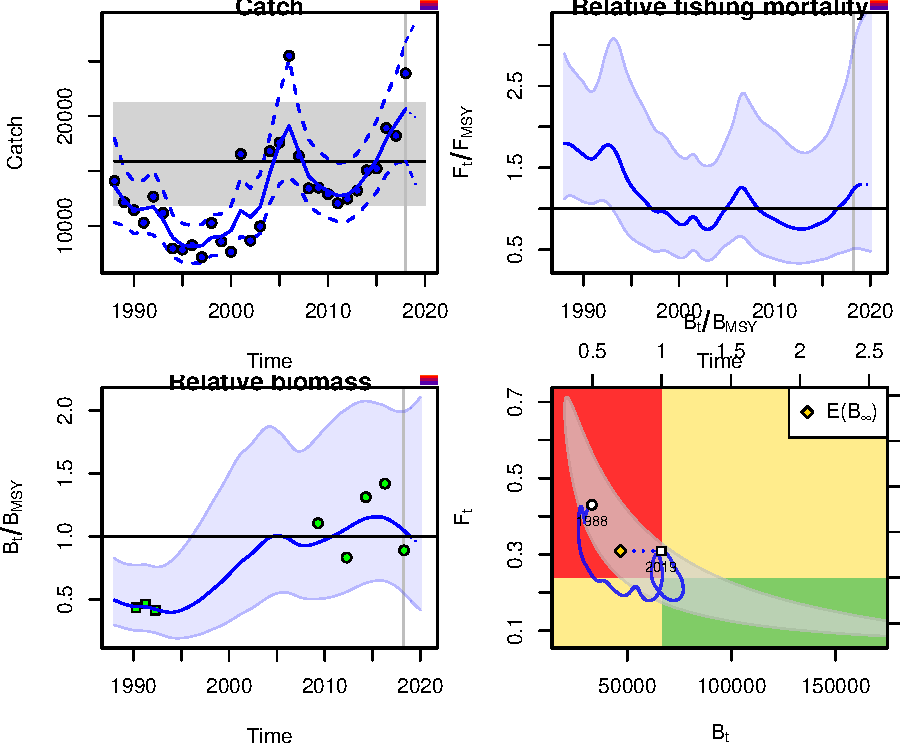
\includegraphics{aru.27.123a4_SPiCT_WD_files/figure-latex/fit_scenario4-2.pdf}

\begin{Shaded}
\begin{Highlighting}[]
\ControlFlowTok{if}\NormalTok{ (converged) \{}
  \KeywordTok{plotspict.diagnostic}\NormalTok{(fit_AC)}
  \KeywordTok{plotspict.production}\NormalTok{(fit_AC)}
\NormalTok{\}}
\end{Highlighting}
\end{Shaded}

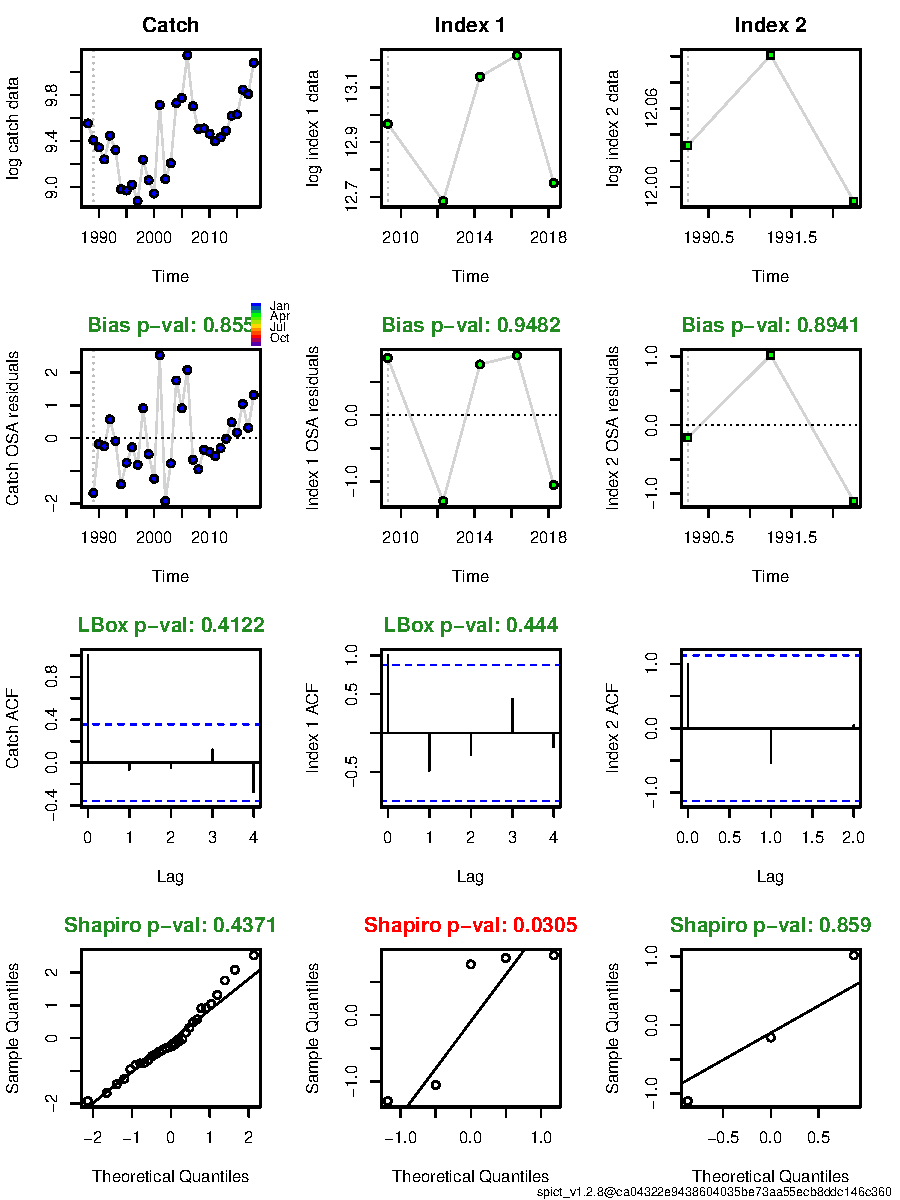
\includegraphics{aru.27.123a4_SPiCT_WD_files/figure-latex/diagnostics_scenario_4-1.pdf}
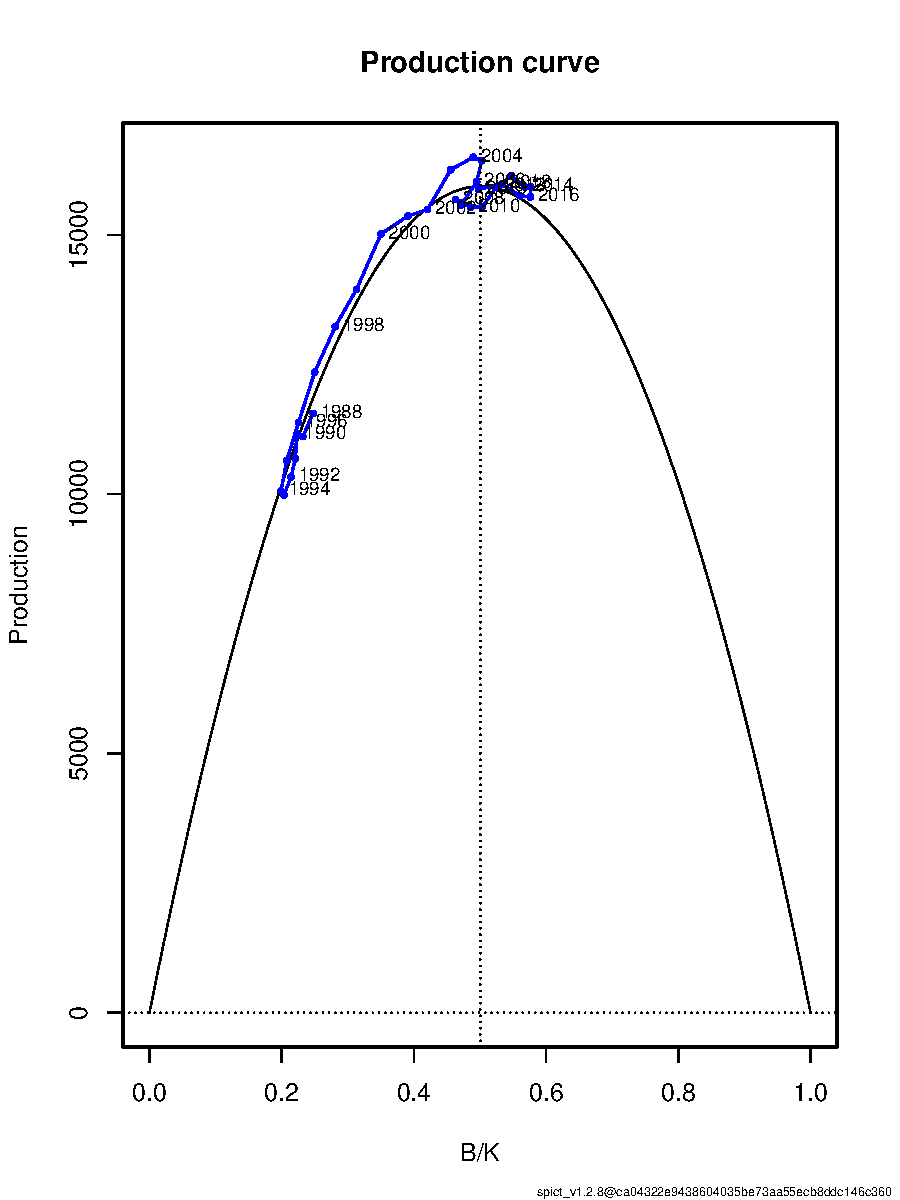
\includegraphics{aru.27.123a4_SPiCT_WD_files/figure-latex/diagnostics_scenario_4-2.pdf}

\begin{Shaded}
\begin{Highlighting}[]
  \CommentTok{## If runretro is TRUE, run and plot the retrospective analysis}
  \CommentTok{## runretro=TRUE}
\ControlFlowTok{if}\NormalTok{ (runretro }\OperatorTok{&}\StringTok{ }\NormalTok{converged) \{}
\NormalTok{    fit_AC <-}\StringTok{ }\KeywordTok{retro}\NormalTok{(fit_AC)}
    \KeywordTok{plotspict.retro}\NormalTok{(fit_AC)}
\NormalTok{  \}}
\end{Highlighting}
\end{Shaded}

\#\#Scenario 5

\begin{longtable}[]{@{}llll@{}}
\caption{Input data for Scenario 5}\tabularnewline
\toprule
\begin{minipage}[b]{0.21\columnwidth}\raggedright
Input data\strut
\end{minipage} & \begin{minipage}[b]{0.20\columnwidth}\raggedright
Name\strut
\end{minipage} & \begin{minipage}[b]{0.15\columnwidth}\raggedright
Range\strut
\end{minipage} & \begin{minipage}[b]{0.33\columnwidth}\raggedright
Notes\strut
\end{minipage}\tabularnewline
\midrule
\endfirsthead
\toprule
\begin{minipage}[b]{0.21\columnwidth}\raggedright
Input data\strut
\end{minipage} & \begin{minipage}[b]{0.20\columnwidth}\raggedright
Name\strut
\end{minipage} & \begin{minipage}[b]{0.15\columnwidth}\raggedright
Range\strut
\end{minipage} & \begin{minipage}[b]{0.33\columnwidth}\raggedright
Notes\strut
\end{minipage}\tabularnewline
\midrule
\endhead
\begin{minipage}[t]{0.21\columnwidth}\raggedright
Catch\strut
\end{minipage} & \begin{minipage}[t]{0.20\columnwidth}\raggedright
Total catch\strut
\end{minipage} & \begin{minipage}[t]{0.15\columnwidth}\raggedright
1988-2018\strut
\end{minipage} & \begin{minipage}[t]{0.33\columnwidth}\raggedright
\strut
\end{minipage}\tabularnewline
\begin{minipage}[t]{0.21\columnwidth}\raggedright
Biomass indices\strut
\end{minipage} & \begin{minipage}[t]{0.20\columnwidth}\raggedright
Shrimp survey\strut
\end{minipage} & \begin{minipage}[t]{0.15\columnwidth}\raggedright
1984--2002\strut
\end{minipage} & \begin{minipage}[t]{0.33\columnwidth}\raggedright
Only october period\strut
\end{minipage}\tabularnewline
\begin{minipage}[t]{0.21\columnwidth}\raggedright
Biomass indices\strut
\end{minipage} & \begin{minipage}[t]{0.20\columnwidth}\raggedright
Acoustic survey\strut
\end{minipage} & \begin{minipage}[t]{0.15\columnwidth}\raggedright
2012--2018\strut
\end{minipage} & \begin{minipage}[t]{0.33\columnwidth}\raggedright
~StoX\strut
\end{minipage}\tabularnewline
\begin{minipage}[t]{0.21\columnwidth}\raggedright
Biomass indices\strut
\end{minipage} & \begin{minipage}[t]{0.20\columnwidth}\raggedright
Acoustic survey\strut
\end{minipage} & \begin{minipage}[t]{0.15\columnwidth}\raggedright
1990-1993\strut
\end{minipage} & \begin{minipage}[t]{0.33\columnwidth}\raggedright
~Monstad\strut
\end{minipage}\tabularnewline
\begin{minipage}[t]{0.21\columnwidth}\raggedright
\strut
\end{minipage} & \begin{minipage}[t]{0.20\columnwidth}\raggedright
\strut
\end{minipage} & \begin{minipage}[t]{0.15\columnwidth}\raggedright
\strut
\end{minipage} & \begin{minipage}[t]{0.33\columnwidth}\raggedright
Default priors\strut
\end{minipage}\tabularnewline
\bottomrule
\end{longtable}

\begin{Shaded}
\begin{Highlighting}[]
\CommentTok{## Choose only the years where the schrimp survey was in October }
\NormalTok{w <-}\StringTok{ }\OperatorTok{!}\KeywordTok{is.na}\NormalTok{(dat}\OperatorTok{$}\NormalTok{northsea_month) }\OperatorTok{&}\StringTok{ }\NormalTok{dat}\OperatorTok{$}\NormalTok{northsea_month }\OperatorTok{==}\StringTok{ }\DecValTok{10}
\NormalTok{w[}\DecValTok{1}\OperatorTok{:}\DecValTok{4}\NormalTok{]<-}\OtherTok{FALSE} \CommentTok{#remove years before 1988 in schrip survey}
\CommentTok{## Choose only the years where the survey was in January or February }
\NormalTok{v <-}\StringTok{ }\OperatorTok{!}\KeywordTok{is.na}\NormalTok{(dat}\OperatorTok{$}\NormalTok{northsea_month) }\OperatorTok{&}\StringTok{ }\NormalTok{dat}\OperatorTok{$}\NormalTok{northsea_month }\OperatorTok\StringTok{ }\KeywordTok{c}\NormalTok{(}\DecValTok{1}\NormalTok{)}\CommentTok{#c(1, 2)}
\CommentTok{## Make the input list}
\NormalTok{inp_NS <-}\StringTok{ }\KeywordTok{list}\NormalTok{(}\DataTypeTok{timeC =}\NormalTok{ dat}\OperatorTok{$}\NormalTok{year,                                      }\CommentTok{## Timing of catch}
               \DataTypeTok{obsC =}\NormalTok{ dat}\OperatorTok{$}\NormalTok{catchTOT,                                   }\CommentTok{## Observed catches dat$year[v] + dat$northsea_month[v] / 12}
               \DataTypeTok{timeI =} \KeywordTok{list}\NormalTok{(dat}\OperatorTok{$}\NormalTok{year[w] }\OperatorTok{+}\StringTok{ }\NormalTok{dat}\OperatorTok{$}\NormalTok{northsea_month[w] }\OperatorTok{/}\StringTok{ }\DecValTok{12}\NormalTok{,dat}\OperatorTok{$}\NormalTok{year}\FloatTok{+3.5}\OperatorTok{/}\DecValTok{12}\NormalTok{, dat}\OperatorTok{$}\NormalTok{year}\OperatorTok{+}\DecValTok{3}\OperatorTok{/}\DecValTok{12}\NormalTok{),}
               \DataTypeTok{obsI =} \KeywordTok{list}\NormalTok{(dat}\OperatorTok{$}\NormalTok{northsea_SA[w],dat}\OperatorTok{$}\NormalTok{norwegian_seaAC,dat}\OperatorTok{$}\NormalTok{Norwegian_seaAC_Monstad),}
               \DataTypeTok{optimiser.control =} \KeywordTok{list}\NormalTok{(}\DataTypeTok{iter.max =} \FloatTok{1e3}\NormalTok{,               }\CommentTok{## Optimiser options }
                                        \DataTypeTok{eval.max =} \FloatTok{1e3}\NormalTok{),              }\CommentTok{## sometimes help converge}
               
               \DataTypeTok{priors =} \KeywordTok{list}\NormalTok{(                                         }\CommentTok{## List of priors (empty, i.e. default priors)}
 \DataTypeTok{logn=}\KeywordTok{c}\NormalTok{(}\KeywordTok{log}\NormalTok{(}\DecValTok{2}\NormalTok{),.}\DecValTok{5}\NormalTok{,}\DecValTok{1}\NormalTok{)}
 \CommentTok{#logbkfrac=c(log(.5),1,1)}
\CommentTok{## see possible priors with list.possible.priors()}
\NormalTok{                 ))}
\CommentTok{## Check input time series, remove missing and zero observations}
\NormalTok{inp_NS <-}\StringTok{ }\KeywordTok{check.inp}\NormalTok{(inp_NS)}
\end{Highlighting}
\end{Shaded}

\begin{verbatim}
## Removing zero, negative, and NAs in  C  series    
## Removing zero, negative, and NAs in  I  series  2  
## Removing zero, negative, and NAs in  I  series  3
\end{verbatim}

\begin{Shaded}
\begin{Highlighting}[]
\CommentTok{## Plot input data}
\KeywordTok{plotspict.data}\NormalTok{(inp_NS)}
\end{Highlighting}
\end{Shaded}

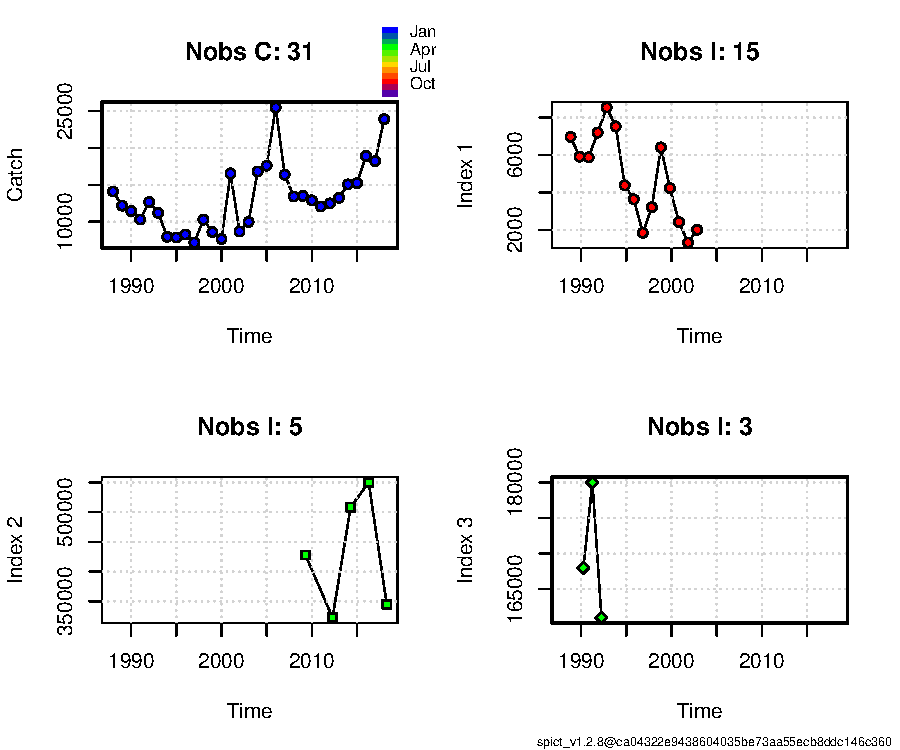
\includegraphics{aru.27.123a4_SPiCT_WD_files/figure-latex/fit_scenario5-1.pdf}

\begin{Shaded}
\begin{Highlighting}[]
\CommentTok{## Fit spict}
\NormalTok{fit_NS <-}\StringTok{ }\KeywordTok{fit.spict}\NormalTok{(inp_NS)}

\CommentTok{## Summary of the fit - in the vignette there is a line-by-line description of that summary}
\NormalTok{fit_NS}
\end{Highlighting}
\end{Shaded}

\begin{verbatim}
## Convergence: 0  MSG: relative convergence (4)
## Objective function at optimum: 24.9215913
## Euler time step (years):  1/16 or 0.0625
## Nobs C: 31,  Nobs I1: 15,  Nobs I2: 5,  Nobs I3: 3
## 
## Priors
##      logn  ~  dnorm[log(2), 0.5^2]
##  logalpha  ~  dnorm[log(1), 2^2]
##   logbeta  ~  dnorm[log(1), 2^2]
## 
## Model parameter estimates w 95% CI 
##             estimate        cilow        ciupp    log.est  
##  alpha1 4.067293e+00    1.0756626 1.537924e+01  1.4029777  
##  alpha2 1.876797e+00    0.4335170 8.125098e+00  0.6295668  
##  alpha3 5.116061e-01    0.0455970 5.740303e+00 -0.6702003  
##  beta   1.151900e+00    0.4271711 3.106187e+00  0.1414126  
##  r      3.336065e-01    0.0378611 2.939515e+00 -1.0977930  
##  rc     3.261774e-01    0.0342092 3.110029e+00 -1.1203139  
##  rold   3.190719e-01    0.0200195 5.085383e+00 -1.1423388  
##  m      2.322892e+04 1204.9062494 4.478215e+05 10.0531535  
##  K      2.824064e+05 3754.5033809 2.124205e+07 12.5511023  
##  q1     1.509100e-02    0.0001121 2.031132e+00 -4.1936593  
##  q2     1.917485e+00    0.0105032 3.500609e+02  0.6510143  
##  q3     4.908080e-01    0.0033167 7.262983e+01 -0.7117023  
##  n      2.045553e+00    0.6838261 6.118934e+00  0.7156681  
##  sdb    1.063387e-01    0.0326205 3.466507e-01 -2.2411261  
##  sdf    1.436392e-01    0.0642778 3.209854e-01 -1.9404505  
##  sdi1   4.325106e-01    0.2685314 6.966241e-01 -0.8381484  
##  sdi2   1.995762e-01    0.0923853 4.311360e-01 -1.6115594  
##  sdi3   5.440350e-02    0.0081871 3.615131e-01 -2.9113265  
##  sdc    1.654580e-01    0.1120487 2.443256e-01 -1.7990379  
##  
## Deterministic reference points (Drp)
##            estimate        cilow        ciupp   log.est  
##  Bmsyd 1.424312e+05 1767.4384920 1.147800e+07 11.866615  
##  Fmsyd 1.630887e-01    0.0171046 1.555015e+00 -1.813461  
##  MSYd  2.322892e+04 1204.9062494 4.478215e+05 10.053154  
## Stochastic reference points (Srp)
##            estimate        cilow        ciupp   log.est rel.diff.Drp  
##  Bmsys 1.394936e+05 1766.4748341 1.101542e+07 11.845774  -0.02105928  
##  Fmsys 1.601562e-01    0.0162055 1.582796e+00 -1.831605  -0.01831021  
##  MSYs  2.233216e+04 1200.8530329 4.153091e+05 10.013783  -0.04015593  
## 
## States w 95% CI (inp$msytype: s)
##                     estimate        cilow        ciupp    log.est  
##  B_2018.25      2.209020e+05 1085.1278426 4.496953e+07 12.3054744  
##  F_2018.25      9.179850e-02    0.0004545 1.854250e+01 -2.3881594  
##  B_2018.25/Bmsy 1.583600e+00    0.5227263 4.797515e+00  0.4597004  
##  F_2018.25/Fmsy 5.731809e-01    0.0106305 3.090506e+01 -0.5565539  
## 
## Predictions w 95% CI (inp$msytype: s)
##                   prediction        cilow        ciupp    log.est  
##  B_2019.00      2.192232e+05 9.924827e+02 4.842283e+07 12.2978458  
##  F_2019.00      9.456820e-02 4.576000e-04 1.954490e+01 -2.3584338  
##  B_2019.00/Bmsy 1.571565e+00 4.780807e-01 5.166107e+00  0.4520718  
##  F_2019.00/Fmsy 5.904748e-01 1.066390e-02 3.269539e+01 -0.5268284  
##  Catch_2019.00  2.049855e+04 1.362292e+04 3.084439e+04  9.9281095  
##  E(B_inf)       1.901561e+05           NA           NA 12.1556007
\end{verbatim}

\begin{Shaded}
\begin{Highlighting}[]
\CommentTok{## If the model converged, it reports convergence as 0}
\CommentTok{## Continue with plotting and diagnostics only if convergence was reached}
\NormalTok{converged <-}\StringTok{ }\NormalTok{fit_NS}\OperatorTok{$}\NormalTok{opt}\OperatorTok{$}\NormalTok{convergence }\OperatorTok{==}\StringTok{ }\DecValTok{0}
\ControlFlowTok{if}\NormalTok{ (converged) \{}
  \CommentTok{## Calculate the One Step Ahead (osa) residuals  }
\NormalTok{  fit_NS <-}\StringTok{ }\KeywordTok{calc.osa.resid}\NormalTok{((fit_NS))}
  
  \CommentTok{## Make a plot showing relative F, relative B, Kobe plot catch }
  \KeywordTok{par}\NormalTok{(}\DataTypeTok{mfrow =} \KeywordTok{c}\NormalTok{(}\DecValTok{2}\NormalTok{,}\DecValTok{2}\NormalTok{),  }\CommentTok{## 2x2 subplots}
      \DataTypeTok{mar =} \KeywordTok{c}\NormalTok{(}\FloatTok{4.1}\NormalTok{, }\FloatTok{4.1}\NormalTok{, }\FloatTok{0.5}\NormalTok{, }\FloatTok{0.5}\NormalTok{)) }\CommentTok{## Change default margins for the plots }
  \KeywordTok{plotspict.catch}\NormalTok{(fit_NS)}
  \KeywordTok{plotspict.ffmsy}\NormalTok{(fit_NS)}
  \KeywordTok{plotspict.bbmsy}\NormalTok{(fit_NS)}
  \KeywordTok{plotspict.fb}\NormalTok{(fit_NS)}
\NormalTok{\}}
\end{Highlighting}
\end{Shaded}

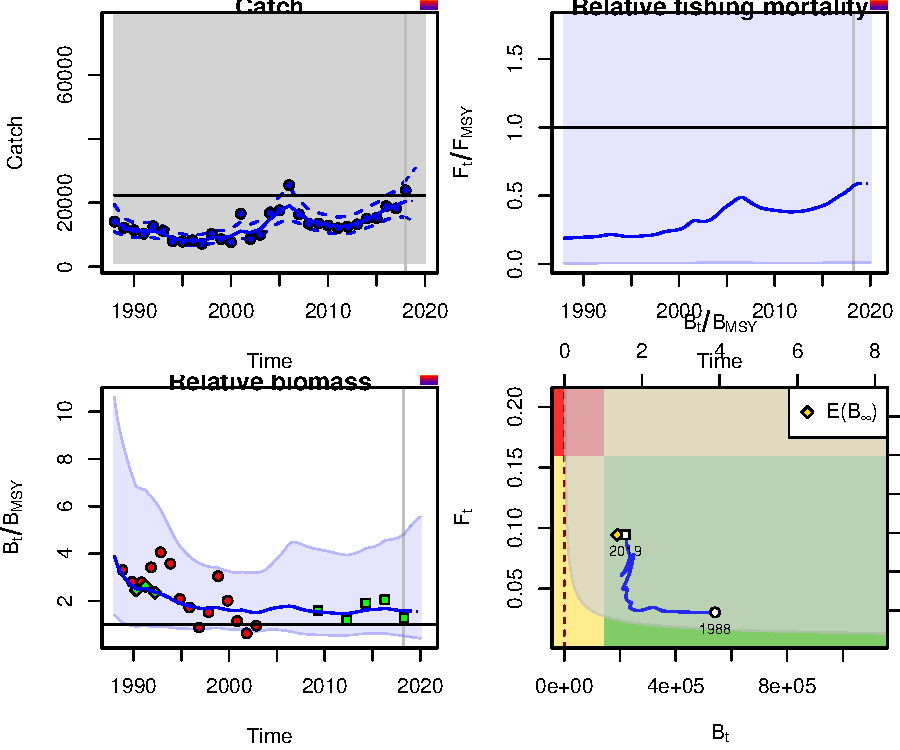
\includegraphics{aru.27.123a4_SPiCT_WD_files/figure-latex/fit_scenario5-2.pdf}

\begin{Shaded}
\begin{Highlighting}[]
\ControlFlowTok{if}\NormalTok{ (converged) \{}
  \KeywordTok{plotspict.diagnostic}\NormalTok{(fit_NS)}
  \KeywordTok{plotspict.production}\NormalTok{(fit_NS)}
\NormalTok{\}}
\end{Highlighting}
\end{Shaded}

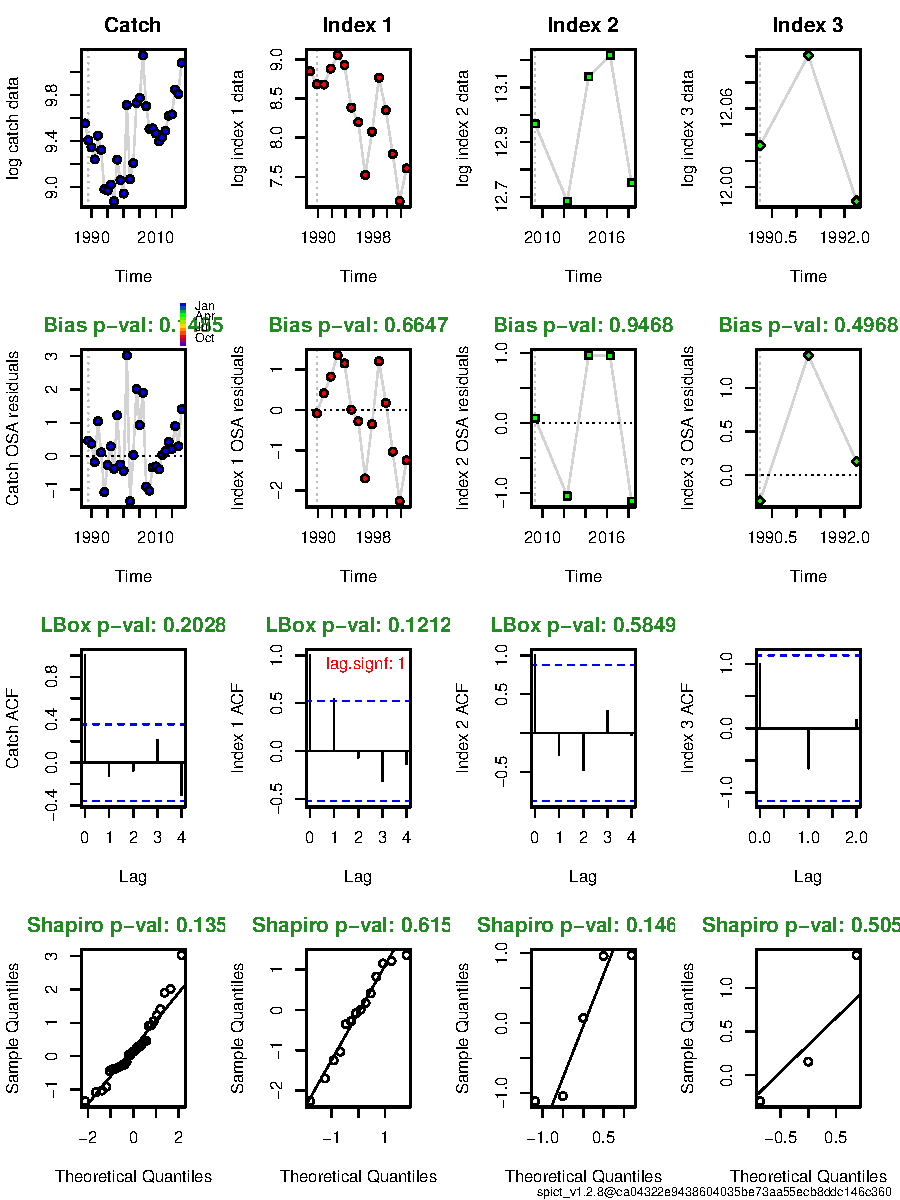
\includegraphics{aru.27.123a4_SPiCT_WD_files/figure-latex/diagnostics_scenario_5-1.pdf}
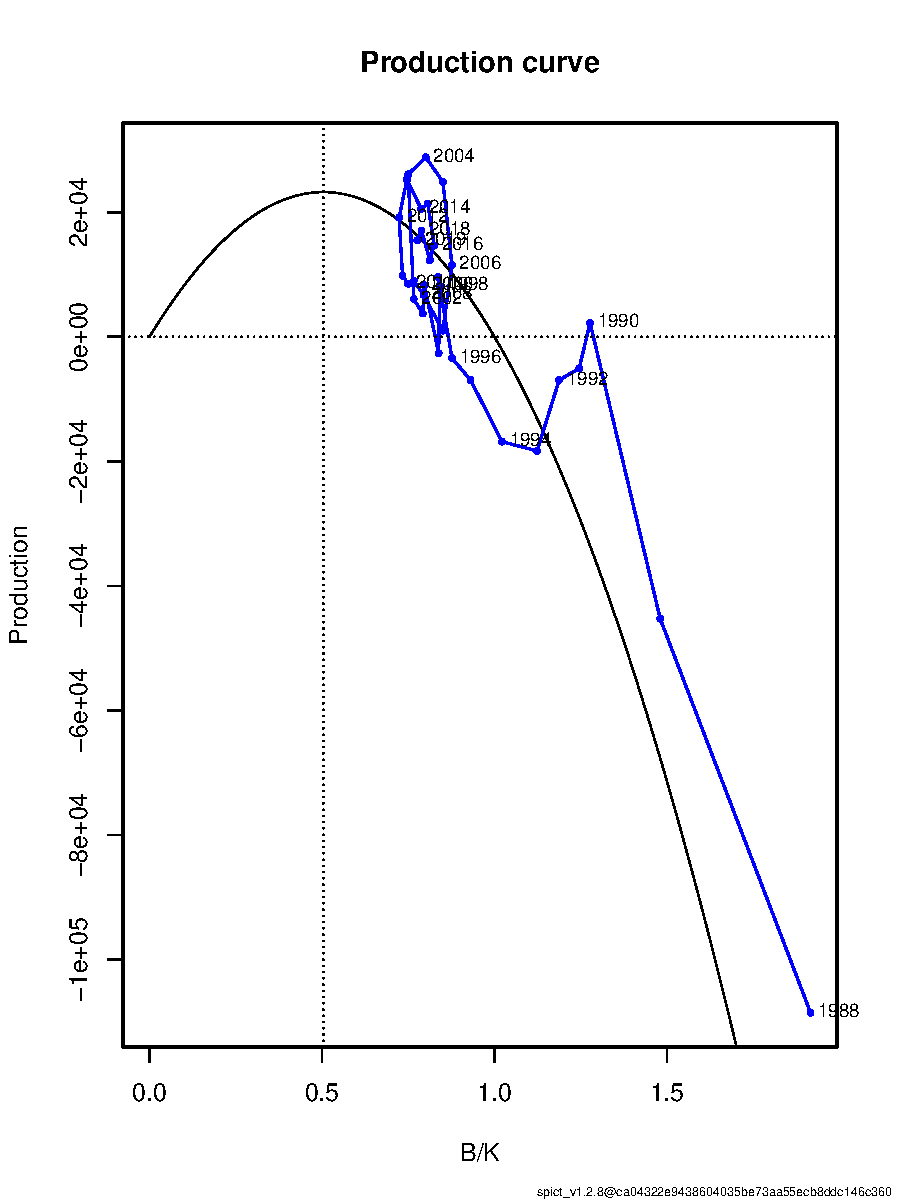
\includegraphics{aru.27.123a4_SPiCT_WD_files/figure-latex/diagnostics_scenario_5-2.pdf}

\begin{Shaded}
\begin{Highlighting}[]
  \CommentTok{## If runretro is TRUE, run and plot the retrospective analysis}
  \CommentTok{#runretro=TRUE}
\ControlFlowTok{if}\NormalTok{ (runretro }\OperatorTok{&}\StringTok{ }\NormalTok{converged) \{}
\NormalTok{    fit_NS <-}\StringTok{ }\KeywordTok{retro}\NormalTok{(fit_NS)}
    \KeywordTok{plotspict.retro}\NormalTok{(fit_NS)}
\NormalTok{  \}}
\end{Highlighting}
\end{Shaded}

\hypertarget{biomass-comparsin-scenario-4-and-5}{%
\subsubsection{Biomass comparsin scenario 4 and
5}\label{biomass-comparsin-scenario-4-and-5}}

\begin{Shaded}
\begin{Highlighting}[]
\NormalTok{bAC <-}\StringTok{ }\KeywordTok{get.par}\NormalTok{(}\DataTypeTok{parname =} \StringTok{"logBBmsy"}\NormalTok{,fit_AC)}
\NormalTok{time <-}\StringTok{ }\KeywordTok{as.numeric}\NormalTok{(}\KeywordTok{rownames}\NormalTok{(bAC))}
\NormalTok{bNS <-}\StringTok{ }\KeywordTok{get.par}\NormalTok{(}\DataTypeTok{parname =} \StringTok{"logBBmsy"}\NormalTok{,fit_NS)}



\NormalTok{meanAC <-}\StringTok{ }\KeywordTok{mean}\NormalTok{(bAC[,}\DecValTok{2}\NormalTok{][time }\OperatorTok{>}\StringTok{ }\DecValTok{2005} \OperatorTok{&}\StringTok{ }\NormalTok{time }\OperatorTok{<}\StringTok{ }\DecValTok{2019}\NormalTok{])}
\NormalTok{meanNS <-}\StringTok{ }\KeywordTok{mean}\NormalTok{(bNS[,}\DecValTok{2}\NormalTok{][time }\OperatorTok{>}\StringTok{ }\DecValTok{2005} \OperatorTok{&}\StringTok{ }\NormalTok{time }\OperatorTok{<}\StringTok{ }\DecValTok{2019}\NormalTok{])}
\NormalTok{ylim <-}\StringTok{ }\KeywordTok{c}\NormalTok{(}\FloatTok{0.3}\NormalTok{, }\FloatTok{1.6}\NormalTok{)}
\KeywordTok{plot}\NormalTok{(time, }\KeywordTok{exp}\NormalTok{(bNS[,}\DecValTok{2}\NormalTok{]) }\OperatorTok{/}\StringTok{ }\KeywordTok{exp}\NormalTok{(meanNS),}\DataTypeTok{col=}\DecValTok{2}\NormalTok{,}\DataTypeTok{type=}\StringTok{"l"}\NormalTok{, }\DataTypeTok{ylim =}\NormalTok{ ylim, }\DataTypeTok{xlim=}\KeywordTok{c}\NormalTok{(}\DecValTok{2005}\NormalTok{,}\DecValTok{2018}\NormalTok{))}
\KeywordTok{lines}\NormalTok{(time, }\KeywordTok{exp}\NormalTok{(bAC[,}\DecValTok{2}\NormalTok{]) }\OperatorTok{/}\StringTok{ }\KeywordTok{exp}\NormalTok{(meanAC))}
\KeywordTok{legend}\NormalTok{(}\StringTok{"bottomright"}\NormalTok{,,}\KeywordTok{c}\NormalTok{(}\StringTok{"NS"}\NormalTok{, }\StringTok{"AC"}\NormalTok{), }\DataTypeTok{col =} \DecValTok{1}\OperatorTok{:}\DecValTok{2}\NormalTok{, }\DataTypeTok{seg.len =} \DecValTok{4}\NormalTok{, }\DataTypeTok{lty =} \DecValTok{1}\NormalTok{)}
\KeywordTok{points}\NormalTok{(dat}\OperatorTok{$}\NormalTok{year, dat}\OperatorTok{$}\NormalTok{norwegian_sea_AC_stox }\OperatorTok{/}\StringTok{ }\KeywordTok{mean}\NormalTok{(dat}\OperatorTok{$}\NormalTok{norwegian_sea_AC_stox, }\DataTypeTok{na.rm =} \OtherTok{TRUE}\NormalTok{))}
\KeywordTok{points}\NormalTok{(dat}\OperatorTok{$}\NormalTok{year, dat}\OperatorTok{$}\NormalTok{norwegian_seaAC }\OperatorTok{/}\StringTok{ }\KeywordTok{mean}\NormalTok{(dat}\OperatorTok{$}\NormalTok{norwegian_seaAC ,}\DataTypeTok{na.rm =} \OtherTok{TRUE}\NormalTok{), }\DataTypeTok{col=}\StringTok{"red"}\NormalTok{)}
\end{Highlighting}
\end{Shaded}

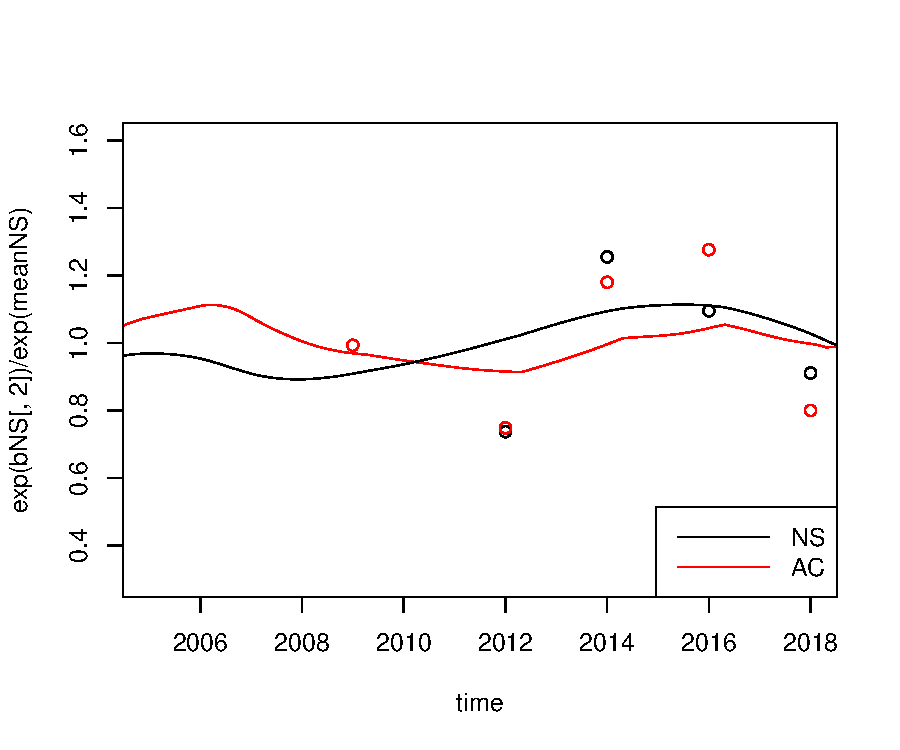
\includegraphics{aru.27.123a4_SPiCT_WD_files/figure-latex/unnamed-chunk-1-1.pdf}

\hypertarget{referneces}{%
\subsection*{Referneces}\label{referneces}}
\addcontentsline{toc}{subsection}{Referneces}

\hypertarget{refs}{}
\leavevmode\hypertarget{ref-Pedersen2016}{}%
Pedersen, Martin W., and Casper W. Berg. 2017. ``A stochastic surplus
production model in continuous time.'' \emph{Fish and Fisheries} 18 (2):
226--43. \url{https://doi.org/10.1111/faf.12174}.

\end{document}
